\documentclass[lang=cn,10pt,bibend=bibtex]{elegantbook}

\title{Project 03: 常微分方程求解器}

\author{Wenchong Huang}
\date{April 10, 2023}

\setcounter{tocdepth}{3}

\logo{figures/logo-blue.jpg}
\cover{figures/cover.jpg}
\usepackage{multirow}
\usepackage{makecell}
\usepackage{xpatch}
\usepackage{tikz}
\makeatletter
% \xpatchcmd{\chapter}
%   {\if@openright\cleardoublepage\else\clearpage\fi}{\par\relax}
%   {}{}
\makeatother

% 本文档命令
\usepackage{array, float}
\newcommand{\ccr}[1]{\makecell{{\color{#1}\rule{1cm}{1cm}}}}

% 修改标题页的橙色带
% \definecolor{customcolor}{RGB}{32,178,170}
% \colorlet{coverlinecolor}{customcolor}

\begin{document}

\maketitle

\frontmatter

\tableofcontents

\mainmatter

\chapter{设计手册}

\section{编译与测试说明}

在根目录下执行
\begin{lstlisting}
  make story
\end{lstlisting}

将自动编译,并生成图片与实验报告。若您想复现报告中的所有数值实验结果,请运行:
\begin{lstlisting}
  make run
\end{lstlisting}

\section{参数说明}

我们采用json文件输入,下面是一个例子

\begin{lstlisting}
  {
    "Problem": "Restricted 3-Body Problem",
    "Method": "Adaptive Radau-IIA",
    "Order": 5,
    "Mass Ratio": 0.012277471,
    "Init": [0.7, 0, 0, 0, -0.403526, 0],
    "T": 12.582604742222023,
    "Periodic": 1,
    "eps": 1e-8,
    "Max Step": 1,
    "Richardson": false,
    "Richardson Error Estimate": true,
    "Output": true,
    "Dense Output": false,
    "Dense-Discrete Output": true,
    "Dense-Discrete Output Step": 0.002
  }
\end{lstlisting}

各参数含义如下:
\begin{itemize}
  \item \verb|Problem|:选择内置方程,可选的方程见1.4节。
  \item \verb|Method|:选择求解方法,可选的方法见1.3节。
  \item \verb|Order|:求解方法的参数(阶数或阶段数,具体见1.3节)。
  \item \verb|Mass Ratio|:限制性三体问题的参数,表示两个大天体的质量之比。
  \item \verb|Init|:初值。
  \item \verb|T|:求解区间$[0,T]$中的参数$T$。
  \item \verb|Periodic|:周期个数(若为周期解请提供该参数,否则请勿提供)。
  \item \verb|eps|:精度的Tolerance,\textbf{自适应方法必须提供该参数,固定步长方法不得提供该参数}。
  \item \verb|Grid Size|:求解结点数$n$,步长取为$T/n$,\textbf{固定步长方法必须提供该参数,自适应方法不得提供该参数}。
  \item \verb|Max Step|:自适应方法的最大步长控制值,可以不提供,默认为$T/100$。
  \item \verb|Richardson Error Estimate|:是否使用Richardson外插法作误差估计(开启后将进行额外的$2n$步求解)。
  \item \verb|Convergence Analysis|:是否估计收敛阶(对于周期解,开启后将进行额外的$2n$步求解;对于非周期解,需要与上一个参数同时开启,将进行额外的$2n$与$4n$步求解)。
  \item \verb|Output|:是否输出求解结点上的计算结果。
  \item \verb|Dense Output|:是否输出每一段区间的插值多项式。
  \item \verb|Dense Discrete Output|:是否根据插值多项式等距离取点输出。
  \item \verb|Dense Discrete Output Step|:根据插值多项式等距离取点输出的步长,默认为$0.01$。
\end{itemize}

\section{方法列表}

我们的求解器支持的线性多步法如下表所示,表中的“方法名称”即求解器用于识别方法的字符串。

\begin{table}[H]
  \centering
  \renewcommand\arraystretch{0.9}
  \begin{tabular}{cccc|cc|ccc}
    \small
  方法名称          & 简称        & 计算类型                   &  步长类型         & 步数 & 阶数  & 零稳定 & A-稳定   \\ \hline
  Adams-Bashforth  & AB$p$        & 显式                     &  固定        &  $p$   &  $p$    &   是   &              \\
  Adams-Moulton  & AM$p$\;\;$(p\geq 2)$   & 隐式                             &  固定        &  $p-1$   &  $p$    &   是   &   $p\leq 2$时     \\
  BDF  & BDF$p$     & 隐式           &  固定         &  $p$   &  $p$    &   $p\leq 6$时   &     $p\leq 2$时
  \end{tabular}
\end{table}
\vspace{-.8em}

支持的RK方法如下表所示,表中的“方法名称”即求解器用于识别方法的字符串。

\begin{table}[H]
  \centering
  \renewcommand\arraystretch{0.9}
  \begin{tabular}{cccc|cc|ccc}
    \small
  方法名称          & 简称         & 计算类型                  &  步长类型         & 阶段数 & 阶数  & A-稳 & B-稳 & L-稳  \\ \hline
  Classical RK  & CLRK           & 显式                  &  固定        &  $4$   &  $4$    &      &      &            \\
  ESDIRK  & ESDIRK & 隐式  &  固定        &  $6$   &  $4$    &   是   &   是   &    是   \\
  % ESDIRK: R(z) = 28*z^4+32*z^3-384*z^2-768z+3072 / -3*z^5+60*z^4-480*z^3+1920*z^2-3840z+3072
  Gauss-Legendre  & GLRK$s$          & 隐式              &  固定         &  $s$   &  $2s$    &   是   &   是   &      \\
  Radau-IIA  & RIIARK$s$             & 隐式              &  固定         &  $s$   &  $2s-1$    &   是   &  是   &   是   \\
  Fehlberg  &  FB4(5)      & 显式    &  自适应       &  $6$   & $4$  &        &      &         \\
  Dormand-Prince  &  DOPRI5   & 显式       &  自适应       &  $7$   & $5$  &        &      &     \\    
  Dormand-Prince 8(7)  &  DOPRI8     & 显式     &  自适应       &  $13$   & $8$  &        &      &     \\    
  Adaptive ESDIRK  & A-ESDIRK & 隐式  &  自适应       &  $6$   &  $4$    &   是   &   是   &    是   \\
  Adaptive Gauss-Legendre & A-GLRK$s$  & 隐式                       &  自适应         &  $s$   &  $2s$    &   是   &   是   &      \\
  Adaptive Radau-IIA & A-RIIARK$s$     & 隐式                       &  自适应         &  $s$   &  $2s-1$    &   是   &  是   &   是   
  \end{tabular}
\end{table}
\vspace{-1em}

凡是带阶数参数的方法,我们都没有内置系数表,而是通过公式计算系数,因此我们不对$s$或$p$的最大取值做限制。但是用户将阶数设置得过高时,实际效果可能反而不如较低阶的方法。

\vspace{-1.2em}
\section{内置方程说明}

\subsection{限制性三体问题}

这是讲义11.7节的测试方程,将\verb|"Problem"|参数设为\verb|"Restricted 3-Body Problem"|即可直接使用。你需要提供参数\verb|"Mass Ratio"|,表示两个大天体的质量之比。在\verb|samples|文件夹中,我们提供了四个测试轨道,命名为\verb|orbits1-4.json|,四个轨道如下。

\begin{figure}[H]
  \centering
  \begin{minipage}[t]{0.36\linewidth}
      \centering
      \includegraphics[width=0.95\linewidth]{figures/0-1.eps}
      \caption*{\small 轨道一}
  \end{minipage}
  \hspace{2em}
  \begin{minipage}[t]{0.36\linewidth}
      \centering
      \includegraphics[width=0.95\linewidth]{figures/0-2.eps}
      \caption*{\small 轨道二}
  \end{minipage}
\end{figure}

\begin{figure}[H]
  \centering
  \begin{minipage}[t]{0.36\linewidth}
    \centering
    \includegraphics[width=0.95\linewidth]{figures/0-3.eps}
    \caption*{\small 轨道三}
  \end{minipage}
  \hspace{2em}
  \begin{minipage}[t]{0.36\linewidth}
      \centering
      \includegraphics[width=0.95\linewidth]{figures/0-4.eps}
      \caption*{\small 轨道四}
  \end{minipage}
\end{figure}

轨道一来自Hairer的经典教材\cite{1987Solving},可以维持至少5个周期,需要较高阶的计算方法,例如我们提供的$5$阶段$9$阶A-RIIARK方法。轨道二可以维持至少5个周期,并不需要非常高阶的方法。轨道三因为距离月球较远,退化成了绕地卫星问题,因此轨道相对稳定,只要精度不要太差,大部分方法都能计算至少15个周期。轨道四的数据来自NASA官网\footnote{\url{https://ssd.jpl.nasa.gov/tools/periodic_orbits.html}}。

我们生成了这些轨道的动态视频,您可以在线观看\footnote{\url{https://www.bilibili.com/video/BV1GM4y1t7av/}\label{fn:视频}}。\textbf{我们将以轨道一与轨道二作为样本,测试各方法的收敛阶数,并通过轨道一的测试观察自适应方法的显著优势。}

\subsection{等质量一般三体问题}

这是三颗等质量恒星在互相的引力作用下运动的方程,将\verb|"Problem"|参数设为\verb|"3-Body Problem"|即可直接使用。初值共有$18$个变量,依次表示三个恒星的空间坐标、三个恒星的初速度。在\verb|samples|文件夹中,我们提供了三个测试轨道,命名为\verb|orbits5-7.json|,其中两个轨道如下。

\begin{figure}[H]
  \centering
  \begin{minipage}[t]{0.42\linewidth}
    \centering
    \includegraphics[width=0.95\linewidth]{figures/0-5.eps}
    \caption*{\small 轨道五}
  \end{minipage}
  \hspace{2em}
  \begin{minipage}[t]{0.42\linewidth}
      \centering
      \includegraphics[width=0.95\linewidth]{figures/0-6.eps}
      \caption*{\small 轨道六}
  \end{minipage}
\end{figure}

这两个轨道由李晓明等人于2017年发现\cite{XiaoMing2017More}。我们生成了这些轨道的动态视频,您可以在线观看\footref{fn:视频}。该方程仅供观赏,不参与数值实验中的测试。

\subsection{稳定性方程}

这个方程是经典的稳定性方程:
\begin{equation}
  u'=\lambda u,\quad u(0)=1.
\end{equation}

其精确解为$u(t)=e^{\lambda t}$,我们的内置参数为$\lambda=-10^{6}$,将\verb|"Problem"|参数设为\verb|"Stability Problem"|即可直接使用。这个方程可以体现数值方法的稳定性:

\begin{itemize}
  \item 不稳定方法:除非步长极小,否则仅需几步,数值解就发散到$\infty$。
  \item A稳定方法:不论步长为多少,数值解始终有界,模长递减收敛至$0$,收敛速度不能保证,可能高频振荡。
  \item L稳定方法:具有A稳定方法的表现,且迅速收敛至$0$,高频振荡将被抑制。
\end{itemize}

\textbf{在数值实验中,我们将使用这个方程验证各方法的稳定性。}

\subsection{Van der Pol方程}

这个方程的表达式如下:
\begin{equation}
  u''=\lambda (1-u^2)u'-u,\quad u(0)=2,\quad u'(0)=0.
\end{equation}

它没有解析解。我们的内置参数为$\lambda=1000$,将\verb|"Problem"|参数设为\verb|"Van der Pol Problem"|即可直接使用。方程的数值解如下图所示。

\begin{figure}[H]
  \centering
  \includegraphics[width=0.5\linewidth]{figures/0-7.eps}
\end{figure}

它是一个典型的刚性方程,使用固定步长方法几乎无法求解,除非步长极小。自适应步长的求解方法也并非都适用于该方程,采用显式方法需要的步数非常多,求解速度很慢,只有自适应步长的隐式方法才能快速求解这个方程。

\textbf{在数值实验中,我们将使用这个方程比较自适应步长的显式方法与隐式方法。}

\section{自定义方程说明}

如果您想要自定义方程,请编写自己的代码,在头文件中包含\verb|"IVP.h"|,您的方程函数需要继承下述基类。
\begin{lstlisting}
  class TimeFunction{
    public:
        virtual ColVector operator () (const ColVector &x, const double &t) const = 0;
    };
\end{lstlisting}

您需要完成虚函数\verb|operator ()|,这表示您的方程$\mathbf{u}'(\mathbf{x},t)=\mathbf{f}(\mathbf{x},t)$中的函数$\mathbf{f}$。

您可以使用下面的代码创建求解器并求解方程。
\begin{lstlisting}
  auto& factory = TimeIntegratorFactory::Instance();
  auto solver = factory.createTimeIntegrator("Radau-IIA", 4); //替换成您需要的方法
  solver->solveWithInfo(*f, x0, T, GridSize, true);           //true表示进行误差估计
  solver->output("result.txt");                               //将结果输出到文件
  solver->denseOutput("result-dense.txt");                    //将结果的插值多项式输出到文件
\end{lstlisting}

更多用法请参考\verb|solve.cpp|。

\section{类设计与继承关系}

我们以\verb|TimeIntegrator|为基类,派生出了各种方法。为了充分复用代码,我们设计了一系列继承关系:

\vspace{-1em}
\begin{center}
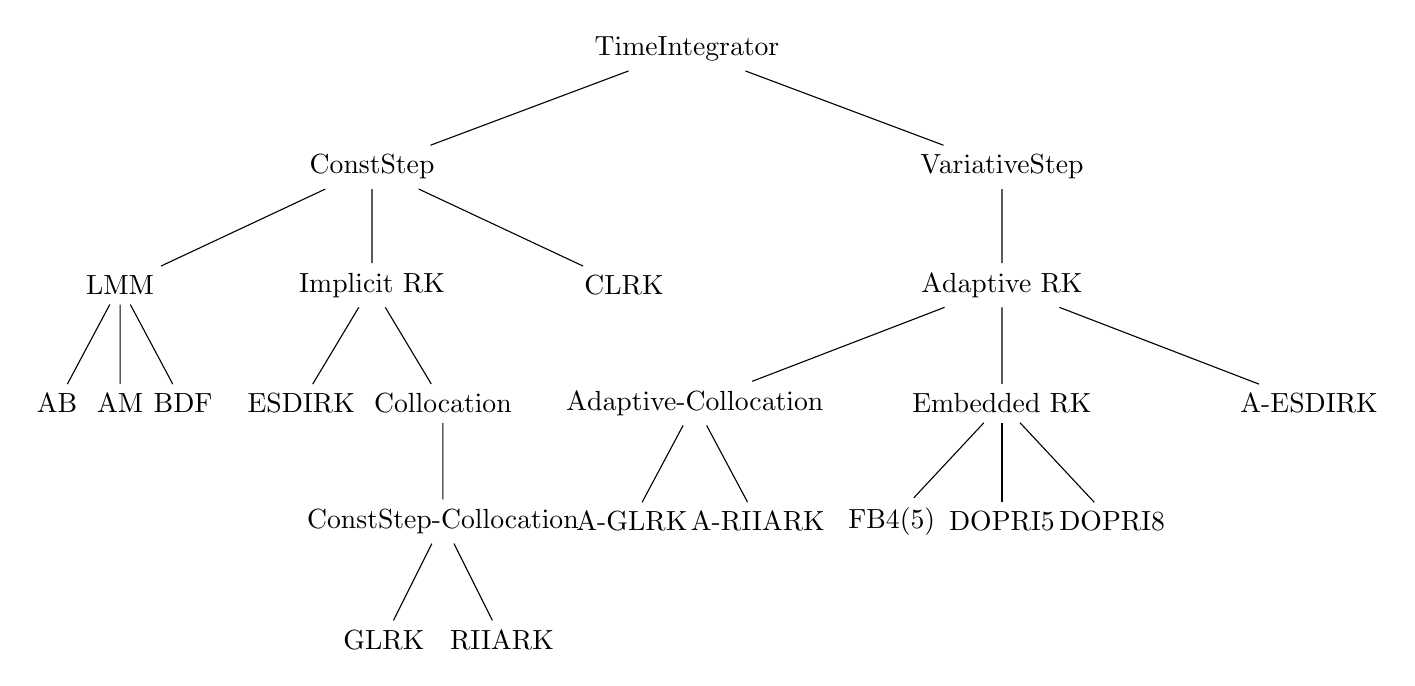
\begin{tikzpicture}
  \node {TimeIntegrator} [sibling distance = 8cm]
    child {node {ConstStep} [sibling distance = 3.2cm]
      child {node {LMM} [sibling distance = 0.8cm]
        child {node {AB}}
        child {node {AM}}
        child {node {BDF}}
      }
      child {node {Implicit RK} [sibling distance = 1.8cm]
        child {node {ESDIRK}}
        child {node {Collocation} [sibling distance = 1.5cm]
          child {node {ConstStep-Collocation}
            child {node {GLRK}}
            child {node {RIIARK}}
          }
        }
      }
      child {node {CLRK}}
    }
    child {node {VariativeStep}[sibling distance = 1.8cm]
      child {node {Adaptive RK} [sibling distance = 3.9cm]
        child {node {Adaptive-Collocation}[sibling distance = 1.6cm]
          child {node {A-GLRK}}
          child {node {A-RIIARK}}
        }
        child {node {Embedded RK}[sibling distance = 1.4cm]
          child {node {FB4(5)}}
          child {node {DOPRI5}}
          child {node {DOPRI8}}
        }
        child {node {A-ESDIRK}}
      }
    };
\end{tikzpicture}
\end{center}

上面的树状图中,有一个多继承关系没有画出:因为除了步长控制,\verb|ConstStep-Collocation|与\verb|Adaptive-Co| \verb|llocation|的一步求解是一样的,因此共同继承了一个Collocation方法的一步求解器。注意,上面的图仅表继承关系,名称并不是代码中类的名称,但大致相同。

对于求解接口,基类提供固定步长与自适应步长两种接口,定义为虚函数。在固定步长求解器基类中禁用自适应步长求解方法,在自适应步长求解器基类中禁用固定步长求解方法。

\verb|IVP|中内置了工厂\verb|TimeIntegratorFactory|,这是一个单例类,设计如下:

\begin{lstlisting}
  class TimeIntegratorFactory{
    public:
        using CreateTimeIntegratorCallBack = TimeIntegrator* (*)(int);
    private:
        using CallbackMap = std::map<std::string, CreateTimeIntegratorCallBack>;
    public:
        bool registerTimeIntegrator(const std::string &ID, CreateTimeIntegratorCallBack createFn);
        bool unregisterTimeIntegrator(const std::string &ID);
        TimeIntegrator* createTimeIntegrator(const std::string &ID, const int &order);
    private:
        CallbackMap callbacks_;
    private:
        TimeIntegratorFactory() = default;
        TimeIntegratorFactory(const TimeIntegratorFactory&) = default;
        TimeIntegratorFactory& operator = (const TimeIntegratorFactory&) = default;
        ~TimeIntegratorFactory() = default;
    public:
        static TimeIntegratorFactory& Instance();
  };
\end{lstlisting}

求解器的注册利用\verb|__attribute__((constructor))|属性,在主函数开始之前执行。用户只需包含头文件\verb|IVP.h|,使用工厂方法\verb|createTimeIntegrator|创建求解器即可。

\chapter{方法实现与数值实验}

\section{经典RK方法}

\subsection{收敛性测试}

在本文中,我们均以限制性三体问题作为收敛性测试的例子。方程与参数、初值见讲义11.7节。

使用经典RK方法,令步长为$\frac{T}{n}$,取不同的$n$,将$T$时刻的数值解与初始点比较误差。对轨道一测试如下。

\vspace{-.5em}
\begin{table}[htbp]
  \centering
  \renewcommand\arraystretch{1.1}
  \begin{tabular}{cc|cccc|c}
  \multicolumn{2}{c|}{$n\;(\times 10^5)$}                  & 1 & 2 & 4 & 8  & 收敛阶 \\ \hline
  \multicolumn{1}{c|}{\multirow{4}{*}{$T$时刻误差}} & \multicolumn{1}{c|}{$u_1$} &  $1.04\times 10^{-6}$  & $6.32\times 10^{-8}$  & $3.89\times 10^{-9}$  & $2.40\times 10^{-10}$    &  $4.02$   \\
  \multicolumn{1}{c|}{}                         & \multicolumn{1}{c|}{$u_2$} &  $3.27\times 10^{-6}$     & $1.98\times 10^{-7}$  & $1.22\times 10^{-8}$  & $7.51\times 10^{-10}$    &  $4.02$   \\
  \multicolumn{1}{c|}{}                         & \multicolumn{1}{c|}{$u_4$} &  $5.33\times 10^{-4}$     & $3.23\times 10^{-5}$  & $1.99\times 10^{-6}$  & $1.22\times 10^{-7}$     &  $4.02$   \\
  \multicolumn{1}{c|}{}                         & \multicolumn{1}{c|}{$u_5$} &  $1.62\times 10^{-4}$     & $9.83\times 10^{-6}$  & $6.06\times 10^{-7}$  & $3.74\times 10^{-8}$     &  $4.02$  \\ \hline
  \multicolumn{2}{c|}{求解时间(s)} & 0.158 & 0.327 & 0.597 & 1.22 & 
  \end{tabular}
\end{table}
\vspace{-.5em}

对轨道二测试如下,这里的收敛阶用Richardson外插法估计。

\vspace{-.5em}
\begin{table}[htbp]
  \centering
  \renewcommand\arraystretch{1.1}
  \begin{tabular}{cc|ccc|c}
  \multicolumn{2}{c|}{$n$}                         & 450 & 900 & 1800 & 收敛阶 \\ \hline
  \multicolumn{1}{c|}{\multirow{4}{*}{与$2n$步的解在$T$时刻的误差}}    & \multicolumn{1}{c|}{$u_1$} & 0.0173229  & 0.000558742  & 1.57643e-05  & $5.15$  \\
  \multicolumn{1}{c|}{}                         & \multicolumn{1}{c|}{$u_2$} &  0.0196696    &  0.000638166  & 2.07028e-05  & $4.94$   \\
  \multicolumn{1}{c|}{}                         & \multicolumn{1}{c|}{$u_4$} &  0.0670598     & 0.00236742  & 6.64987e-05  & $5.16$ \\
  \multicolumn{1}{c|}{}                         & \multicolumn{1}{c|}{$u_5$} &  0.0386287     & 0.00114744  & 3.2626e-05  & $5.14$  \\ \hline
  \multicolumn{2}{c|}{求解时间(s)} & 0.00199 & 0.00128 & 0.00302 &   
  \end{tabular}
\end{table}
\vspace{-.5em}

要想绘制出仅用肉眼无法辨别的图像,轨道一需要取$n=15000$,轨道二需要取$n=800$,绘制的图像如下。

\vspace{-.8em}
\begin{figure}[H]
  \centering
  \begin{minipage}[t]{0.4\linewidth}
      \centering
      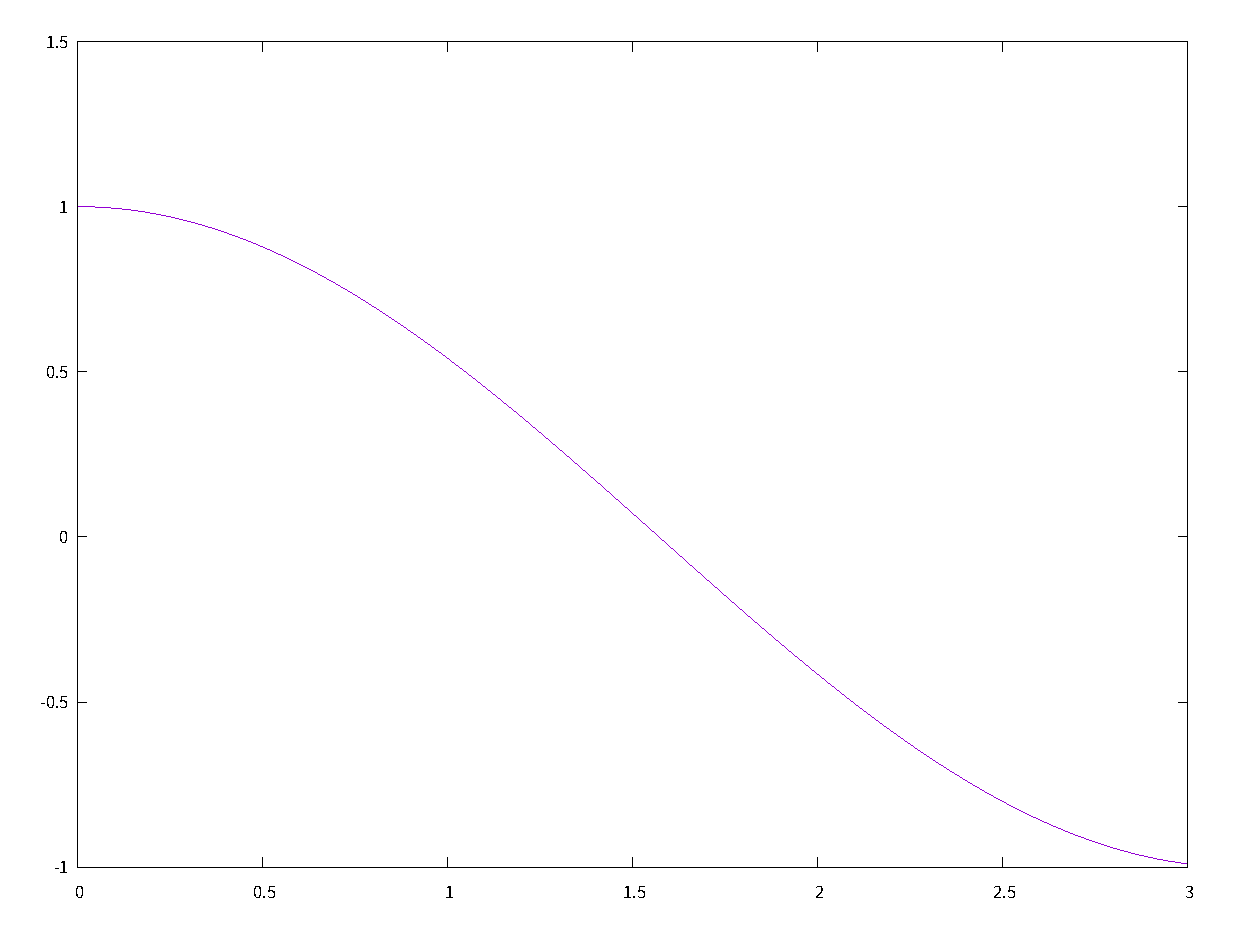
\includegraphics[width=0.95\linewidth]{figures/1-1.eps}
      \caption*{轨道一,$n=15000$}
  \end{minipage}
  \hspace{2em}
  \begin{minipage}[t]{0.4\linewidth}
      \centering
      \includegraphics[width=0.95\linewidth]{figures/1-2.eps}
      \caption*{轨道二,$n=800$}
  \end{minipage}
\end{figure}
\vspace{-2em}

\subsection{稳定性测试}
\vspace{-.8em}

使用稳定性方程(1.1)测试经典RK方法,求解区间为$[0,1]$,步长为$\frac{1}{n}$,结果如下表。当数值解为-nan时我们称为“溢出”,当数值解的绝对值首次小于$10^{-5}$时,我们称为“收敛”。

\begin{table}[htbp]
  \centering
  \renewcommand\arraystretch{1.1}
  \begin{tabular}{c|cccc}
    $n$ & $3.5\times 10^5$ & $3.6\times 10^5$ & $3.7\times 10^5$ \\ \hline
    $T$时刻的数值解 & -nan & $1.97\times 10^{-306}$ & $1.86\times 10^{-307}$\\
    溢出或收敛所用步数 & 6445 & 1016 & 93 \\
    溢出或收敛的时刻 & 0.01841 & 0.002822 & 0.000251
  \end{tabular}
\end{table}
\vspace{-.8em}
\subsection{结论}
\vspace{-.8em}

收敛性测试的结果表明,经典RK方法的累积误差约$O(k^4)$,是一个四阶精度的方法。

稳定性测试的结果表明,经典RK方法不具有A稳定性,且绝对稳定区域较小,因此不适用于刚性方程。

\section{ESDIRK方法}

事实上,ESDIRK是一族方法,我们仅实现了其中一个,该方法的Butcher表在讲义中已经给出。我们这里指出,讲义中给出的这个ESDIRK方法具有L稳定性,见参考文献\cite{2003Additive}。

\subsection{隐式方法的计算过程}

考虑到ESDIRK是隐式方法,我们需要解四个非线性方程,每个方程形如:
\begin{equation}
  \mathbf{y}_i=\mathbf{f}(\mathbf{a}+c\mathbf{y}_i,b).
\end{equation}

其中$\mathbf{a},b,c$是可以事先计算好的常量,$\mathbf{y}_i$是$m$维向量,$m$为微分方程的变量个数。对于这样的方程,我们给出\textbf{第一种计算方法}:

\begin{enumerate}[itemindent=1em]
  \item $\mathbf{y}_i\gets \mathbf{0}$.
  \item $\hat{\mathbf{y}}_i\gets \mathbf{y}_i,\;\mathbf{y}_i\gets\mathbf{f}(\mathbf{a}+c\mathbf{y}_i,b)$.
  \item 若$||\hat{\mathbf{y}}_i-\mathbf{y}_i||<\varepsilon$,结束,否则返回步骤2.
\end{enumerate}

实践告诉我们,上述计算过程在很多刚性方程中并不能收敛。因此我们还要给出\textbf{第二种方法}:

\begin{enumerate}[itemindent=1em]
  \item 设$\mathbf{g}(\mathbf{x})=\mathbf{f}(\mathbf{a}+c\mathbf{x},b)-\mathbf{x}$.
  \item 以$\mathbf{0}$为初值,使用牛顿迭代法求$\mathbf{g}(\mathbf{x})$的零点.
\end{enumerate}

上面两种方法中,我们优先使用第一种,当第一种方法迭代50次而无法收敛时,再采取第二种方法,若还不收敛,则求解失败。

事实上,我们还面临一个巨大的问题——\textbf{数值微分的不稳定性}。我们采用第二种方法时,牛顿迭代需要求Jacobi矩阵,并对其做LU分解,这对微分的精度有较高的要求。要求用户提供导函数的表达式是不现实的,限制性三体问题的求导对人类来说过于复杂。Jorge Nocedal在他的著作\cite{1999NumOpt}中给出了一种解析求导的方法,基本思路为将函数分解为一系列初等函数进行求导,但这需要用户提供计算路线图。

在我们的求解器中,仍然采用数值微分格式:
\begin{equation}
  f'(x)\approx \frac{f(x+h)-f(x-h)}{2h}.
\end{equation}

确定$h$的取值非常困难,起初我们为了精度,将$h$取得很小,然而这带来了严重的数值不稳定性,这导致牛顿迭代难以收敛。在王何宇老师的建议下,我们根据参考资料\cite{叶兴德2008数值分析基础},确定了$h$的最优取值为
\begin{equation}
  h=\sqrt[3]{\frac{3\mathbf{\epsilon}}{M}}.
\end{equation}

其中$\mathbf{\epsilon}$表示机器精度,$M=\sup |f'''(x)|$。在我们的求解器中,$h$被估计为$3\times 10^{-6}$。

另一个问题是——\textbf{Jacobi矩阵奇异}。在某些点处可能会发生这个情况,导致牛顿迭代失败。为此,可以使用Gill-Murray修正牛顿法\cite{1974Newton}或其它方法。但由于我们并不是做专门的优化求解器,因此我们只做粗略修正:
\begin{equation}
  J\gets J+0.01I.
\end{equation}

经过测试,用上述步骤计算隐式方法的迭代格式,在数值上较为稳定,在四个内置方程中均表现良好。

\subsection{收敛性测试}

使用ESDIRK方法,令步长为$\frac{T}{n}$,取不同的$n$,将$T$时刻的数值解与初始点比较误差。对轨道一测试如下。

\begin{table}[htbp]
  \centering
  \renewcommand\arraystretch{1.1}
  \begin{tabular}{cc|cccc|c}
  \multicolumn{2}{c|}{$n\;(\times 10^5)$}                  & 0.5 & 1 & 2 & 4  & 收敛阶 \\ \hline
  \multicolumn{1}{c|}{\multirow{4}{*}{$T$时刻误差}} & \multicolumn{1}{c|}{$u_1$} & $5.78\times 10^{-6}$ &  $3.62\times 10^{-7}$  & $2.27\times 10^{-8}$  & $1.42\times 10^{-9}$    &  $4.00$   \\
  \multicolumn{1}{c|}{}                         & \multicolumn{1}{c|}{$u_2$} & $1.88\times 10^{-5}$ &  $1.18\times 10^{-6}$     & $7.39\times 10^{-8}$  & $4.63\times 10^{-9}$    &  $4.00$   \\
  \multicolumn{1}{c|}{}                         & \multicolumn{1}{c|}{$u_4$} & $3.06\times 10^{-3}$ &  $1.92\times 10^{-4}$     & $1.20\times 10^{-5}$  & $7.54\times 10^{-7}$     &  $4.00$   \\
  \multicolumn{1}{c|}{}                         & \multicolumn{1}{c|}{$u_5$} & $8.94\times 10^{-4}$ &  $5.64\times 10^{-5}$     & $3.53\times 10^{-6}$  & $2.22\times 10^{-7}$     &  $4.00$  \\ \hline
  \multicolumn{2}{c|}{求解时间(s)} & 0.519 & 1.06 & 2.18 & 4.41 & 
  \end{tabular}
\end{table}

对轨道二测试如下,这里的收敛阶用Richardson外插法估计。

\begin{table}[htbp]
  \centering
  \renewcommand\arraystretch{1.1}
  \begin{tabular}{cc|ccc|c}
  \multicolumn{2}{c|}{$n$}                         & 500 & 1000 & 2000  & 收敛阶 \\ \hline
  \multicolumn{1}{c|}{\multirow{4}{*}{与$2n$步的解在$T$时刻的误差}}    & \multicolumn{1}{c|}{$u_1$} & 0.000844317  & 3.19044e-05  & 1.16815e-06   &   $4.77$  \\
  \multicolumn{1}{c|}{}                         & \multicolumn{1}{c|}{$u_2$} &  0.000722844    & 2.50061e-05  & 7.46045e-07   &   $5.07$   \\
  \multicolumn{1}{c|}{}                         & \multicolumn{1}{c|}{$u_4$} &  0.00365792     & 0.000138021  & 5.08278e-06   &   $4.76$ \\
  \multicolumn{1}{c|}{}                         & \multicolumn{1}{c|}{$u_5$} &  0.00167582     & 6.32808e-05  & 2.29493e-06   &   $4.79$  \\ \hline
  \multicolumn{2}{c|}{求解时间(s)} & 0.0144 & 0.0196 & 0.0342  &   
  \end{tabular}
\end{table}

要想绘制出仅用肉眼无法辨别的图像,轨道一需要取$n=9000$,轨道二需要取$n=700$,绘制的图像如下。

\begin{figure}[H]
  \centering
  \begin{minipage}[t]{0.35\linewidth}
      \centering
      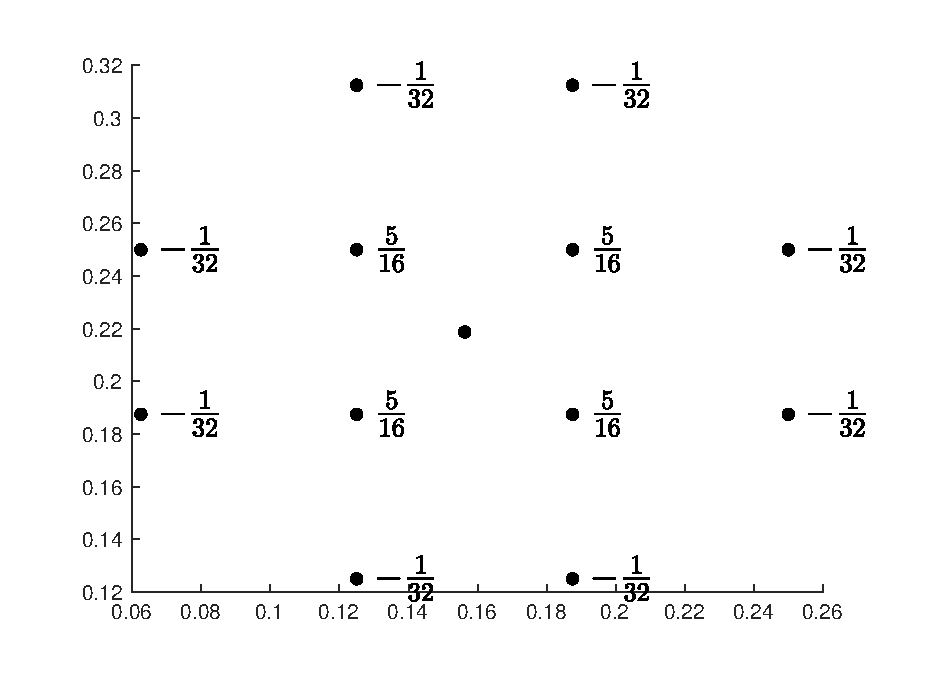
\includegraphics[width=0.95\linewidth]{figures/2-1.eps}
      \caption*{轨道一,$n=9000$}
  \end{minipage}
  \hspace{2em}
  \begin{minipage}[t]{0.35\linewidth}
      \centering
      \includegraphics[width=0.95\linewidth]{figures/2-2.eps}
      \caption*{轨道二,$n=700$}
  \end{minipage}
\end{figure}

与经典RK方法相比,虽然ESDIRK的计算相对准确,因此点数取得少一些,但是求解时间却更长。

\subsection{稳定性测试}

使用稳定性方程(1.1)测试ESDIRK方法,求解区间为$[0,1]$,步长为$\frac{1}{n}$,结果如下表。当数值解为-nan时我们称为“溢出”,当数值解的绝对值首次小于$10^{-5}$时,我们称为“收敛”。

\begin{table}[htbp]
  \centering
  \renewcommand\arraystretch{1.1}
  \begin{tabular}{c|cccc}
    $n$ & $10$ & $100$ & $1000$ & $10000$\\ \hline
    $T$时刻的数值解 & $1.19\times 10^{-24}$ & $6.87\times 10^{-24}$ & $8.00\times 10^{-21}$ & $2.21\times 10^{-20}$\\
    溢出或收敛所用步数 & 2 & 2 & 3 & 6\\
    溢出或收敛的时刻 & 0.2 & 0.02 & 0.003 & 0.0005
  \end{tabular}
\end{table}

注意,这里$T$时刻的数值解不具备比较意义,因为隐式方法的求解基于迭代,而当解的绝对误差达到机器精度时,迭代会立刻停止,并不会像显式方法一样继续下降到$10^{-308}$级别。

事实上,对于讲义上的刚性方程(11.95),取$\lambda=-10^6$时,不论取步长为多少,ESDIRK方法总能得到稳定解。这个测试我们不在本文展示。

\subsection{结论}

收敛性测试的结果表明,ESDIRK方法的一步误差约$O(k^5)$,累积误差约$O(k^4)$,是一个四阶精度的方法。

稳定性测试的结果表明,ESDIRK方法具有A稳定性、L稳定性,具有一定的求解刚性方程的能力。改造成自适应方法后,可能会适用于刚性方程(见A-ESDIRK的测试)。

\vspace{-1.5em}
\section{Gauss-Legendre方法}
\vspace{-.5em}

\subsection{方法实现与L稳定性分析}

在GLRK方法的实现中,我们并没有直接使用讲义上的Butcher表,而是使用数值代数的方法求多项式(2.5)的根,再由讲义上的(11.150)计算$A$与$\mathbf{b}$,这样我们就可以支持任意的$s$。例如当$s=5$时,我们生成的Butcher表如下。

\begin{table}[htbp]
  \centering
  \begin{tabular}{c|ccccc}
    0.0469101 & 0.0592317 & -0.0195704 & 0.0112544 & -0.00559379 & 0.00158811\\
    0.230765 & 0.128151 & 0.119657 & -0.0245921 & 0.0103183 & -0.00276899\\
    0.5 & 0.113776 & 0.260005 & 0.142222 & -0.0206903 & 0.00468715\\
    0.769235 & 0.121232 & 0.228996 & 0.309037 & 0.119657 & -0.00968756\\
    0.95309  & 0.116875 & 0.244908 & 0.27319 & 0.258885 & 0.0592317\\ \hline
     & 0.118463 & 0.239314 & 0.284444 & 0.239314 & 0.118463
  \end{tabular}
\end{table}

\vspace{-1em}

GLRK是隐式方法,且$\mathbf{y}_i$与$\mathbf{y}_1,...,\mathbf{y}_s$均有关,因此不能像ESDIRK一样逐个迭代以求出$\mathbf{y}_i$,而是需要一起迭代。我们给出\textbf{第一种方法}:

\begin{enumerate}[itemindent=1em]
  \item $\mathbf{y}_i\gets \mathbf{f}(\mathbf{U}^n,t_n),\;(i=1,...,s)$.
  \item 对$i=1,...,s$依次做:$\hat{\mathbf{y}}_i\gets \mathbf{y}_i,\;\mathbf{y}_i\gets\mathbf{f}(\mathbf{U}^n+k\sum_{j=1}^s a_{ij}\mathbf{y}_j, t_n+c_ik)$.
  \item 若$\max_{i=1}^s ||\hat{\mathbf{y}}_i-\mathbf{y}_i||<\varepsilon$,结束,否则返回步骤2.
\end{enumerate}

实践告诉我们,上述计算过程在很多刚性方程中并不能收敛。因此我们还要给出\textbf{第二种方法}:牛顿迭代法。两种方法中,我们优先使用第一种,当第一种方法迭代50次而无法收敛时,再采取第二种方法,若还不收敛,则求解失败。

这里我们牛顿迭代法要求解的是一个$sm$元函数的零点,$m$为微分方程的变量个数。每次迭代需要计算Jacobi矩阵并做LU分解,一个牛顿步的计算的代价高达$O((sm)^3)$。在刚性方程的求解中,刚性区域的牛顿迭代占用了大部分的时间。

讲义的Example 11.265指出,GLRK$3$不具有L稳定性,事实上我们有更一般的结论:

\begin{theorem}
  对任意的$s\geq 1$,GLRK$s$均具有A稳定性、B稳定性,但不具有L稳定性。
\end{theorem}

\begin{proof}
  根据\cite{2002Solving}第IV章习题3,一个配点法具有L稳定性的必要条件是存在$c_i=1$. GLRK的$c_1,...,c_s$是多项式:
  \begin{equation}
    P_s(t)=\frac{(s!)^2}{(2s)!}\sum_{j=0}^s (-1)^{s-j}\binom{s}{j}\binom{s+j}{j}t^j.
  \end{equation}

  的所有根。存在$c_i=1$意味着$P_s(1)=0$,然而:
  \begin{equation*}
    P_s(1)=\frac{(s!)^2}{(2s)!}\sum_{j=0}^s (-1)^{s-j}\binom{s}{j}\binom{s+j}{j}=\frac{(s!)^2}{(2s)!}\neq 0.
  \end{equation*}

  矛盾,因此不存在$c_i=1$,所以GLRK不具有L稳定性。A稳定性与B稳定性见讲义中的定理11.283。
\end{proof}

\vspace{-.8em}
\subsection{收敛性测试}
\vspace{-.8em}

使用GLRK$s$方法,令步长为$\frac{T}{n}$,取不同的$n$,对轨道一测试,将$T$时刻的数值解与初始点比较误差,当$s=1$时,即一阶段二阶GLRK方法,结果如下。

\vspace{-.5em}
\begin{table}[H]
  \centering
  \renewcommand\arraystretch{0.9}
  \begin{tabular}{cc|cccc|c}
  \multicolumn{2}{c|}{$n\;(\times 10^6)$}                  & 2.5 & 5 & 10 & 20  & 收敛阶 \\ \hline
  \multicolumn{1}{c|}{\multirow{4}{*}{$T$时刻误差}} & \multicolumn{1}{c|}{$u_1$} & $1.21\times 10^{-5}$ &  $3.02\times 10^{-6}$  & $7.54\times 10^{-7}$  & $1.88\times 10^{-7}$    &  $2.00$   \\
  \multicolumn{1}{c|}{}                         & \multicolumn{1}{c|}{$u_2$} & $3.82\times 10^{-5}$ &  $9.55\times 10^{-6}$     & $2.39\times 10^{-6}$  & $5.97\times 10^{-7}$    &  $2.00$   \\
  \multicolumn{1}{c|}{}                         & \multicolumn{1}{c|}{$u_4$} & $6.24\times 10^{-3}$ &  $1.56\times 10^{-3}$     & $3.89\times 10^{-4}$  & $9.72\times 10^{-5}$     &  $2.00$   \\
  \multicolumn{1}{c|}{}                         & \multicolumn{1}{c|}{$u_5$} & $1.86\times 10^{-3}$ &  $4.68\times 10^{-4}$     & $1.17\times 10^{-4}$  & $2.93\times 10^{-5}$     &  $2.00$  \\ \hline
  \multicolumn{2}{c|}{求解时间(s)} & 5.88 & 10.1 & 20.6 & 41.6 & 
  \end{tabular}
\end{table}
\vspace{-.8em}

$s=2$结果如下。

\vspace{-.8em}
\begin{table}[H]
  \centering
  \renewcommand\arraystretch{0.9}
  \begin{tabular}{cc|cccc|c}
  \multicolumn{2}{c|}{$n\;(\times 10^4)$}                  & 2.5 & 5 & 10 & 20  & 收敛阶 \\ \hline
  \multicolumn{1}{c|}{\multirow{4}{*}{$T$时刻误差}} & \multicolumn{1}{c|}{$u_1$} & $6.79\times 10^{-5}$ &  $4.23\times 10^{-6}$  & $2.65\times 10^{-7}$  & $1.66\times 10^{-8}$    &  $4.00$   \\
  \multicolumn{1}{c|}{}                         & \multicolumn{1}{c|}{$u_2$} & $1.95\times 10^{-4}$ &  $1.24\times 10^{-5}$     & $7.80\times 10^{-7}$  & $4.88\times 10^{-8}$    &  $4.00$   \\
  \multicolumn{1}{c|}{}                         & \multicolumn{1}{c|}{$u_4$} & $3.23\times 10^{-2}$ &  $2.03\times 10^{-3}$     & $1.27\times 10^{-4}$  & $7.97\times 10^{-6}$     &  $4.00$   \\
  \multicolumn{1}{c|}{}                         & \multicolumn{1}{c|}{$u_5$} & $9.92\times 10^{-3}$ &  $6.56\times 10^{-4}$     & $4.13\times 10^{-5}$  & $2.58\times 10^{-6}$     &  $4.00$  \\ \hline
  \multicolumn{2}{c|}{求解时间(s)} & 0.219 & 0.349 & 0.567 & 1.48 & 
  \end{tabular}
\end{table}

$s=3$结果如下。

\vspace{-.8em}
\begin{table}[htbp]
  \centering
  \renewcommand\arraystretch{0.9}
  \begin{tabular}{cc|cccc|c}
  \multicolumn{2}{c|}{$n\;(\times 10^4)$}                  & 0.875 & 1.75 & 3.5 & 7  & 收敛阶 \\ \hline
  \multicolumn{1}{c|}{\multirow{4}{*}{$T$时刻误差}} & \multicolumn{1}{c|}{$u_1$} & $1.25\times 10^{-4}$ &  $1.75\times 10^{-6}$  & $2.70\times 10^{-8}$  & $4.20\times 10^{-10}$    &  $6.01$   \\
  \multicolumn{1}{c|}{}                         & \multicolumn{1}{c|}{$u_2$} & $3.79\times 10^{-4}$ &  $5.49\times 10^{-6}$     & $8.46\times 10^{-8}$  & $1.32\times 10^{-9}$    &  $6.01$   \\
  \multicolumn{1}{c|}{}                         & \multicolumn{1}{c|}{$u_4$} & $6.35\times 10^{-2}$ &  $8.95\times 10^{-4}$     & $1.38\times 10^{-5}$  & $2.15\times 10^{-7}$     &  $6.01$   \\
  \multicolumn{1}{c|}{}                         & \multicolumn{1}{c|}{$u_5$} & $1.69\times 10^{-2}$ &  $2.72\times 10^{-4}$     & $4.20\times 10^{-6}$  & $6.54\times 10^{-8}$     &  $6.01$  \\ \hline
  \multicolumn{2}{c|}{求解时间(s)} & 0.0833 & 0.151 & 0.298 & 0.522 & 
  \end{tabular}
\end{table}
\vspace{-1em}

对轨道二测试,这里的收敛阶用Richardson外插法估计,$s=1$结果如下。

\vspace{-.8em}
\begin{table}[H]
  \centering
  \renewcommand\arraystretch{0.9}
  \begin{tabular}{cc|cccc|c}
  \multicolumn{2}{c|}{$n\;(\times 10^4)$}                         & 1 & 2 & 4 & 8  & 收敛阶 \\ \hline
  \multicolumn{1}{c|}{\multirow{4}{*}{\makecell{与$2n$步的解\\在$T$时刻的误差}}}    & \multicolumn{1}{c|}{$u_1$} & 0.000221967  & 5.55177e-05  & 1.3881e-05  & 3.47036e-06   &   $2.00$  \\
  \multicolumn{1}{c|}{}                         & \multicolumn{1}{c|}{$u_2$} &  7.95868e-05    & 1.99551e-05  & 4.99243e-06  & 1.24833e-06   &  $2.00$   \\
  \multicolumn{1}{c|}{}                         & \multicolumn{1}{c|}{$u_4$} &  0.00100695     & 0.000251523  & 6.28674e-05  & 1.5716e-05   & $2.00$ \\
  \multicolumn{1}{c|}{}                         & \multicolumn{1}{c|}{$u_5$} &  0.000404512     & 0.000101212  & 2.53082e-05  & 6.32738e-06   & $2.00$  \\ \hline
  \multicolumn{2}{c|}{求解时间(s)} & 0.0348 & 0.0691 & 0.109 & 0.211 &   
  \end{tabular}
\end{table}
\vspace{-1em}

$s=2$结果如下。

\vspace{-.8em}
\begin{table}[H]
  \centering
  \renewcommand\arraystretch{0.9}
  \begin{tabular}{cc|cccc|c}
  \multicolumn{2}{c|}{$n\;(\times 10^3)$}                         & 1 & 2 & 4 & 8  & 收敛阶 \\ \hline
  \multicolumn{1}{c|}{\multirow{4}{*}{\makecell{与$2n$步的解\\在$T$时刻的误差}}}    & \multicolumn{1}{c|}{$u_1$} & 2.63427e-05  & 1.65245e-06  & 1.03375e-07  & 6.46248e-09   &   $4.00$  \\
  \multicolumn{1}{c|}{}                         & \multicolumn{1}{c|}{$u_2$} &  8.14391e-06    & 5.10769e-07  & 3.19459e-08  & 1.99689e-09   &  $4.00$   \\
  \multicolumn{1}{c|}{}                         & \multicolumn{1}{c|}{$u_4$} &  0.000119076     & 7.46844e-06  & 4.67207e-07  & 2.92074e-08   & $4.00$ \\
  \multicolumn{1}{c|}{}                         & \multicolumn{1}{c|}{$u_5$} &  4.80285e-05     & 3.01287e-06  & 1.8848e-07  & 1.17829e-08   & $4.00$  \\ \hline
  \multicolumn{2}{c|}{求解时间(s)} & 0.0339 & 0.0563 & 0.0822 & 0.145 &   
  \end{tabular}
\end{table}
\vspace{-1em}

$s=3$结果如下。

\vspace{-.8em}
\begin{table}[H]
  \centering
  \renewcommand\arraystretch{0.9}
  \begin{tabular}{cc|cccc|c}
  \multicolumn{2}{c|}{$n$}                         & 450 & 900 & 1800 & 3600  & 收敛阶 \\ \hline
  \multicolumn{1}{c|}{\multirow{4}{*}{\makecell{与$2n$步的解\\在$T$时刻的误差}}}    & \multicolumn{1}{c|}{$u_1$} & 2.9731e-06  & 4.75577e-08  & 7.47275e-10  & 1.18147e-11   &   $5.99$  \\
  \multicolumn{1}{c|}{}                         & \multicolumn{1}{c|}{$u_2$} &  6.89595e-07    & 1.09705e-08  & 1.72299e-10  & 2.54906e-12   &  $6.02$   \\
  \multicolumn{1}{c|}{}                         & \multicolumn{1}{c|}{$u_4$} &  1.33968e-05     & 2.14281e-07  & 3.36701e-09  & 5.32073e-11   & $5.99$ \\
  \multicolumn{1}{c|}{}                         & \multicolumn{1}{c|}{$u_5$} &  5.42078e-06    & 8.67106e-08  & 1.36245e-09  & 2.15747e-11   & $5.99$  \\ \hline
  \multicolumn{2}{c|}{求解时间(s)} & 0.0322 & 0.0494 & 0.088 & 0.15 &   
  \end{tabular}
\end{table}
\vspace{-1em}

绘图结果如下,$n$均取尽可能小,并保证图像能准确到看不出差异。

\begin{figure}[H]
  \centering
  \begin{minipage}[t]{0.33\linewidth}
      \centering
      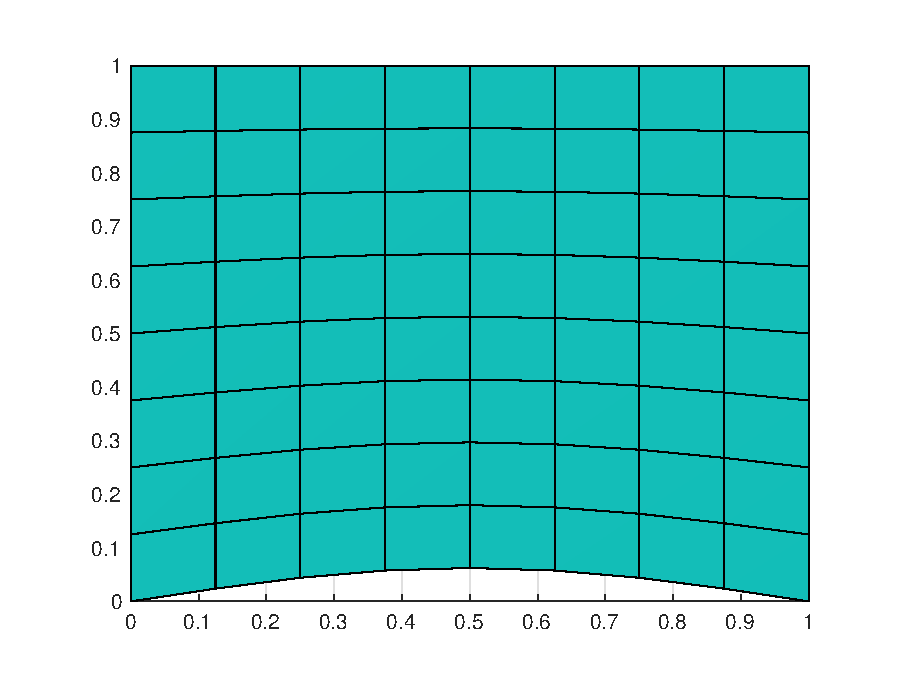
\includegraphics[width=0.95\linewidth]{figures/3-1.eps}
      \caption*{\small $s=1$,$n=110000$,0.358秒}
  \end{minipage}
  \hspace{1em}
  \begin{minipage}[t]{0.33\linewidth}
      \centering
      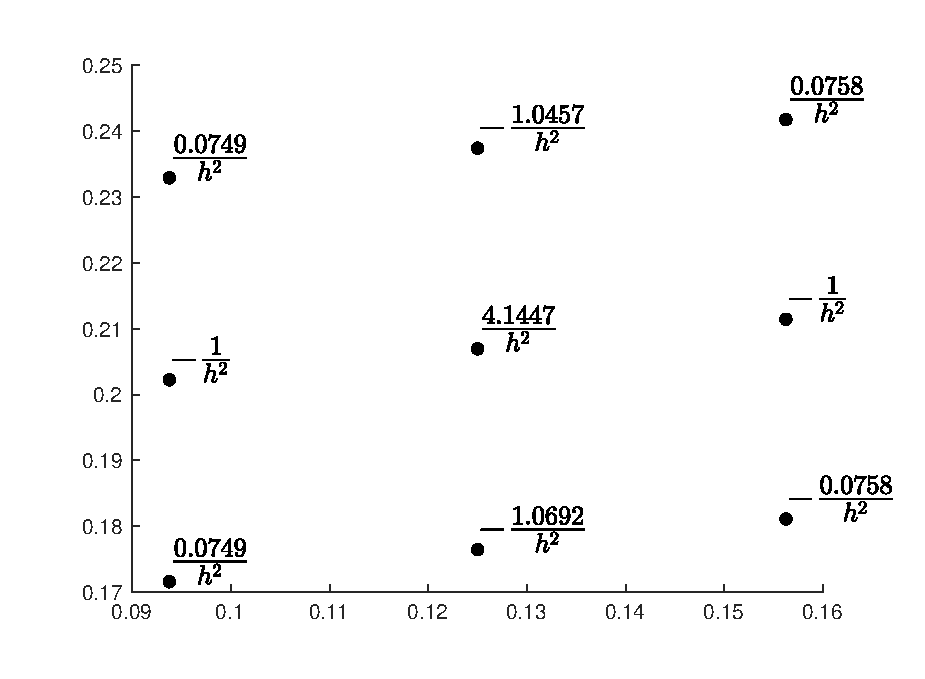
\includegraphics[width=0.95\linewidth]{figures/3-2.eps}
      \caption*{\small $s=1$,$n=3000$,0.0101秒}
  \end{minipage}
  \begin{minipage}[t]{0.33\linewidth}
      \centering
      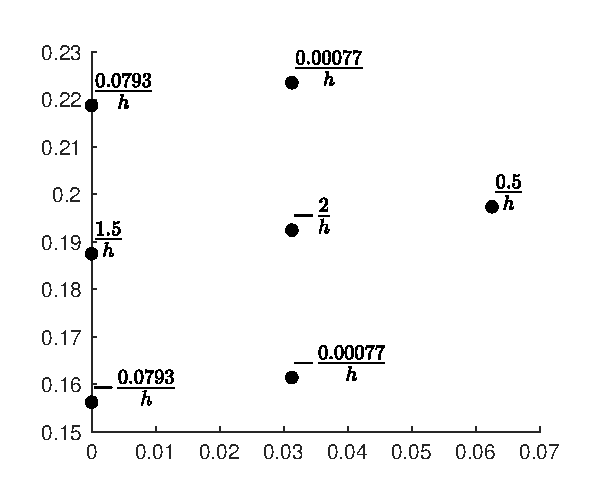
\includegraphics[width=0.95\linewidth]{figures/3-3.eps}
      \caption*{\small $s=2$,$n=9000$,0.0671秒}
  \end{minipage}
  \hspace{1em}
  \begin{minipage}[t]{0.33\linewidth}
    \centering
    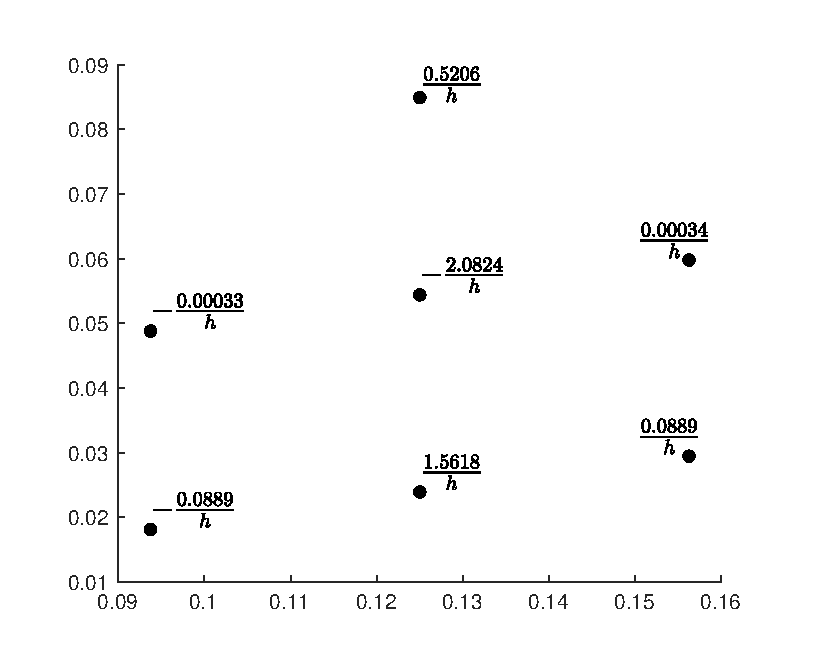
\includegraphics[width=0.95\linewidth]{figures/3-4.eps}
    \caption*{\small $s=2$,$n=320$,0.0043秒}
  \end{minipage}
\end{figure}

\begin{figure}[H]
  \centering
  \begin{minipage}[t]{0.33\linewidth}
      \centering
      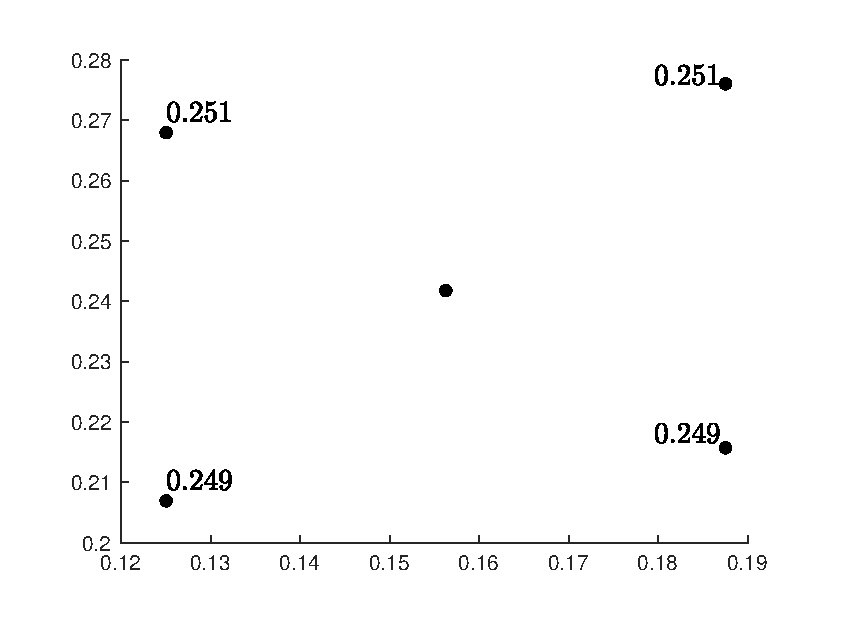
\includegraphics[width=0.95\linewidth]{figures/3-5.eps}
      \caption*{\small $s=3$,$n=3500$,0.0461秒}
  \end{minipage}
  \hspace{1em}
  \begin{minipage}[t]{0.33\linewidth}
      \centering
      \includegraphics[width=0.95\linewidth]{figures/3-6.eps}
      \caption*{\small $s=3$,$n=160$,0.0096秒}
  \end{minipage}
\end{figure}

\subsection{稳定性测试}

使用稳定性方程(1.1)测试GLRK$s$方法$(s=1,2,3)$,求解区间为$[0,1]$,步长为$0.002$,将数值解作图如下。可以看到,数值解始终保持有界,且绝对值随时间递减。但是收敛速度极慢,且$s=1,3$时高频振荡。

\begin{figure}[H]
  \centering
  \begin{minipage}[t]{0.32\linewidth}
      \centering
      \includegraphics[width=0.95\linewidth]{figures/3-7.eps}
      \caption*{$s=1$}
  \end{minipage}
  \hspace{.3em}
  \begin{minipage}[t]{0.32\linewidth}
      \centering
      \includegraphics[width=0.95\linewidth]{figures/3-8.eps}
      \caption*{$s=2$}
  \end{minipage}
  \hspace{.3em}
  \begin{minipage}[t]{0.32\linewidth}
      \centering
      \includegraphics[width=0.95\linewidth]{figures/3-9.eps}
      \caption*{$s=3$}
  \end{minipage}
\end{figure}

\subsection{结论}

收敛性测试的结果表明,GLRK$s$方法的一步误差约$O(k^{2s+1})$,累积误差约$O(k^{2s})$,是一个$2s$阶精度的方法。用户可以将$s$设置得任意大,但不建议超过$5$。

稳定性测试的结果表明,GLRK$s$方法具有A稳定性,不具有L稳定性,求解刚性方程的能力较弱。

\section{Radau-IIA方法}

\subsection{方法介绍与实现}

Radau-IIA方法是一种具有L稳定性的配点法\cite{1969A},事实上,讲义中的Example 11.267就是3阶段5阶Radau-IIA方法。下面我们来构造一般的$s$阶段$2s-1$阶Radau-IIA方法。我们设多项式
\begin{equation}
  P_s(x)=\frac{\text{d}^{s-1}}{\text{d}x^{s-1}} x^{s-1}(x-1)^s.
\end{equation}

Radau-IIA方法的$c_1,...,c_s$是$P_s(x)$的所有根(从小到大排列),再由讲义上的(11.150)计算$A$与$\mathbf{b}$。同样的,我们不内置Butcher表,而是通过数值代数的方法求根,从而可以支持任意大的$s$。

通过上述方法构造好Butcher表后,求解过程与GLRK完全一样。在代码实现时,求解过程被定义在它们共同的父类中。

\subsection{收敛性测试}

使用RIIARK$s$方法,令步长为$\frac{T}{n}$,取不同的$n$,对轨道一测试,将$T$时刻的数值解与初始点比较误差,当$s=2$时,即二阶段三阶Radau-IIA RK方法,结果如下。

\begin{table}[H]
  \centering
  \renewcommand\arraystretch{0.8}
  \begin{tabular}{cc|ccc|c}
  \multicolumn{2}{c|}{$n\;(\times 10^5)$}                  & 1 & 2 & 4  & 收敛阶 \\ \hline
  \multicolumn{1}{c|}{\multirow{4}{*}{$T$时刻误差}} & \multicolumn{1}{c|}{$u_1$} &  $7.52\times 10^{-5}$  & $9.12\times 10^{-6}$  & $1.13\times 10^{-6}$    &  $3.01$   \\
  \multicolumn{1}{c|}{}                         & \multicolumn{1}{c|}{$u_2$} &  $2.34\times 10^{-4}$     & $2.92\times 10^{-5}$  & $3.64\times 10^{-6}$    &  $3.00$   \\
  \multicolumn{1}{c|}{}                         & \multicolumn{1}{c|}{$u_4$} &  $3.88\times 10^{-2}$     & $4.76\times 10^{-3}$  & $5.93\times 10^{-4}$     &  $3.01$   \\
  \multicolumn{1}{c|}{}                         & \multicolumn{1}{c|}{$u_5$} &  $1.07\times 10^{-2}$     & $1.40\times 10^{-3}$  & $1.76\times 10^{-4}$     &  $2.99$  \\ \hline
  \multicolumn{2}{c|}{求解时间(s)} & 0.511 & 1.35 & 3.55 & 
  \end{tabular}
\end{table}

$s=3$结果如下。

\vspace{-.5em}
\begin{table}[H]
  \centering
  \renewcommand\arraystretch{0.8}
  \begin{tabular}{cc|ccc|c}
  \multicolumn{2}{c|}{$n\;(\times 10^4)$}                  & 4 & 8 & 16  & 收敛阶 \\ \hline
  \multicolumn{1}{c|}{\multirow{4}{*}{$T$时刻误差}} & \multicolumn{1}{c|}{$u_1$} &  $3.23\times 10^{-7}$  & $1.00\times 10^{-8}$  & $3.09\times 10^{-10}$    &  $5.02$   \\
  \multicolumn{1}{c|}{}                         & \multicolumn{1}{c|}{$u_2$} &  $1.11\times 10^{-6}$     & $3.43\times 10^{-8}$  & $1.06\times 10^{-9}$    &  $5.01$   \\
  \multicolumn{1}{c|}{}                         & \multicolumn{1}{c|}{$u_4$} &  $1.80\times 10^{-4}$     & $5.58\times 10^{-6}$  & $1.73\times 10^{-7}$     &  $5.01$   \\
  \multicolumn{1}{c|}{}                         & \multicolumn{1}{c|}{$u_5$} &  $5.03\times 10^{-5}$     & $1.56\times 10^{-6}$  & $4.81\times 10^{-8}$     &  $5.02$  \\ \hline
  \multicolumn{2}{c|}{求解时间(s)} & 0.475 & 0.755 & 2.41 & 
  \end{tabular}
\end{table}
\vspace{-.5em}

对轨道二测试,这里的收敛阶用Richardson外插法估计,$s=2$结果如下。

\vspace{-.5em}
\begin{table}[H]
  \centering
  \renewcommand\arraystretch{0.8}
  \begin{tabular}{cc|ccc|c}
  \multicolumn{2}{c|}{$n\;(\times 10^4)$}                         & 2 & 4 & 8 & 收敛阶 \\ \hline
  \multicolumn{1}{c|}{\multirow{4}{*}{一步误差}}    & \multicolumn{1}{c|}{$u_1$} & 3.96162e-06  & 4.95246e-07  & 6.19073e-08   &   $3.00$  \\
  \multicolumn{1}{c|}{}                         & \multicolumn{1}{c|}{$u_2$} &  3.98663e-06    & 4.98329e-07  & 6.22902e-08    &  $3.00$   \\
  \multicolumn{1}{c|}{}                         & \multicolumn{1}{c|}{$u_4$} &  1.68681e-05    & 2.10876e-06  & 2.63602e-07   & $3.00$ \\
  \multicolumn{1}{c|}{}                         & \multicolumn{1}{c|}{$u_5$} &  8.08741e-06    & 1.01098e-06  & 1.26375e-07   & $3.00$  \\ \hline
  \multicolumn{2}{c|}{求解时间(s)} & 0.176 & 0.332 & 0.581 &   
  \end{tabular}
\end{table}
\vspace{-.5em}

$s=3$结果如下。

\vspace{-.5em}
\begin{table}[H]
  \centering
  \renewcommand\arraystretch{0.8}
  \begin{tabular}{cc|ccc|c}
  \multicolumn{2}{c|}{$n\;(\times 10^3)$}           &              2 & 4 & 8  & 收敛阶 \\ \hline
  \multicolumn{1}{c|}{\multirow{4}{*}{一步误差}}    & \multicolumn{1}{c|}{$u_1$}  & 8.75807e-07  & 2.74218e-08  & 8.57287e-10   &   $5.00$  \\
  \multicolumn{1}{c|}{}                         & \multicolumn{1}{c|}{$u_2$}  & 8.80329e-07  & 2.75448e-08  & 8.60868e-10   &  $5.00$   \\
  \multicolumn{1}{c|}{}                         & \multicolumn{1}{c|}{$u_4$}  & 3.73978e-06  & 1.17098e-07  & 3.6609e-09   & $5.00$ \\
  \multicolumn{1}{c|}{}                         & \multicolumn{1}{c|}{$u_5$}  & 1.77721e-06  & 5.56413e-08  & 1.73946e-09   & $5.00$  \\ \hline
  \multicolumn{2}{c|}{求解时间(s)} & 0.0304 & 0.0858 & 0.242 & 
  \end{tabular}
\end{table}
\vspace{-.5em}

绘图结果如下,$n$均取尽可能小,并保证图像能准确到看不出差异。

\begin{figure}[H]
  \centering
  \begin{minipage}[t]{0.32\linewidth}
      \centering
      \includegraphics[width=0.95\linewidth]{figures/4-1.eps}
      \caption*{\small $s=2$,$n=30000$,0.157秒}
  \end{minipage}
  \hspace{1em}
  \begin{minipage}[t]{0.32\linewidth}
      \centering
      \includegraphics[width=0.95\linewidth]{figures/4-2.eps}
      \caption*{\small $s=3$,$n=4500$,0.0527秒}
  \end{minipage}
\end{figure}

\begin{figure}[H]
  \centering
  \begin{minipage}[t]{0.32\linewidth}
      \centering
      \includegraphics[width=0.95\linewidth]{figures/4-3.eps}
      \caption*{\small $s=2$,$n=2200$,0.0573秒}
  \end{minipage}
  \hspace{1em}
  \begin{minipage}[t]{0.32\linewidth}
    \centering
    \includegraphics[width=0.95\linewidth]{figures/4-4.eps}
    \caption*{\small $s=3$,$n=380$,0.0096秒}
  \end{minipage}
\end{figure}

\subsection{稳定性测试}

使用稳定性方程(1.1)测试Radau-IIA方法,求解区间为$[0,1]$,步长为$0.02$,结果如下表。当数值解的绝对值首次小于$10^{-5}$时,我们称为“收敛”。

\begin{table}[htbp]
  \centering
  \renewcommand\arraystretch{1.1}
  \begin{tabular}{c|ccc}
    $s$ & $2$ & $3$ & $4$\\ \hline
    收敛所用步数 & 2 & 2 & 2\\
    收敛的时刻 & 0.04 & 0.04 & 0.04
  \end{tabular}
\end{table}
\vspace{-2em}

\subsection{结论}

收敛性测试的结果表明,$s$阶段Radau-IIA方法的一步误差约$O(k^{2s})$,累积误差约$O(k^{2s-1})$,是一个$2s-1$阶精度的方法。用户可以将$s$设置得任意大,但不建议超过$5$。

稳定性测试的结果表明,Radau-IIA方法具有A稳定性、L稳定性,有求解刚性方程的能力。

\section{Dormand-Prince方法}

\subsection{方法介绍与实现}

我们实现了DOPRI5与DOPRI8两种Dormand-Prince方法,前者是讲义中的方法,后者是matlab的求解器\verb|ode87|采用的方法,是最为流行的高阶数值积分方法。DOPRI8的构造方法与Butcher表见Prince和Dormand的文章\cite{PRINCE198167}。

步长控制采用了讲义Formula 11.235中的方法,它被写在了所有自适应方法的共同基类中。

另外,由于使用Dormand-Prince方法求解非刚性方程时,所需的结点通常很少,这会使我们画出的图看上去不够光滑,因此我们用3阶2次Hermite插值填充结点之间的值,并以0.01的时间间隔输出。

\subsection{非刚性方程测试}

使用限制性三体问题作为样例测试DOPRI5方法。Tolerance从$3.2768\times 10^{-9}$开始,每次减小至原来的$\frac{1}{32}$,观察DOPRI5的步数需要增加至多少。若步数的增长率接近$2$,则可以验证DOPRI5方法具有$5$阶收敛性。轨道一的结果如下表。

\begin{table}[H]
  \centering
  \begin{tabular}{c|cccc|c}
    Tolerance$(\times 10^{-13})$ & 32768 & 1024 & 32 & 1 & 增长率 \\ \hline
    所需步数 & 472 & 944 & 1887 & 3775 & 2.00   \\
    计算时间(s) & 0.00398 & 0.00715  & 0.0128  & 0.0246 & 
  \end{tabular}
\end{table}

轨道二的结果如下表。

\begin{table}[H]
  \centering
  \begin{tabular}{c|cccc|c}
    Tolerance$(\times 10^{-13})$ & 32768 & 1024 & 32 & 1 & 增长率 \\ \hline
    所需步数 & 739 & 1477 & 2953 & 5906 & 2.00   \\
    计算时间(s) & 0.00563 & 0.00979  & 0.0218  & 0.0423 & 
  \end{tabular}
\end{table}

同样地,我们测试DOPRI8方法。Tolerance从$6.5536\times 10^{-9}$开始,每次减小至原来的$\frac{1}{256}$,观察DOPRI8的步数需要增加至多少。若步数的增长率接近$2$,则可以验证DOPRI8方法具有$8$阶收敛性。轨道一结果如下表。

\begin{table}[H]
  \centering
  \begin{tabular}{c|cccc|c}
    Tolerance$(\times 10^{-13})$ & 16777216 & 65536 & 256 & 1 & 增长率 \\ \hline
    所需步数 & 68 & 123 & 230  & 460 & 2.00   \\
    计算时间(s) & 0.0014 & 0.00241  & 0.00478  & 0.00766 & 
  \end{tabular}
\end{table}

轨道二的结果如下表。

\begin{table}[H]
  \centering
  \begin{tabular}{c|cccc|c}
    Tolerance$(\times 10^{-13})$ & 16777216 & 65536 & 256 & 1 & 增长率 \\ \hline
    所需步数 & 107 & 193 & 361 & 723 & 2.00   \\
    计算时间(s) & 0.00234 & 0.00487  & 0.00638  & 0.0121 & 
  \end{tabular}
\end{table}

用DOPRI5与DOPRI8绘制图像,并将求解结点标出,如下。其中Tolerance在轨道一中设为$10^{-4}$,在轨道二中设为$5\times 10^{-6}$。

\begin{figure}[H]
  \centering
  \begin{minipage}[t]{0.34\linewidth}
      \centering
      \includegraphics[width=0.95\linewidth]{figures/5-1.eps}
      \caption*{\small DOPRI5,$n=64$}
  \end{minipage}
  \hspace{1em}
  \begin{minipage}[t]{0.34\linewidth}
      \centering
      \includegraphics[width=0.95\linewidth]{figures/5-2.eps}
      \caption*{\small DOPRI5,$n=171$}
  \end{minipage}
\end{figure}

\begin{figure}[H]
  \centering
  \begin{minipage}[t]{0.34\linewidth}
      \centering
      \includegraphics[width=0.95\linewidth]{figures/5-3.eps}
      \caption*{\small DOPRI8,$n=47$}
  \end{minipage}
  \hspace{1em}
  \begin{minipage}[t]{0.34\linewidth}
      \centering
      \includegraphics[width=0.95\linewidth]{figures/5-4.eps}
      \caption*{\small DOPRI8,$n=95$}
  \end{minipage}
\end{figure}

我们来比较两种方法在长时间尺度下的稳定性。将轨道一的计算周期由原来的$T$增加至$5T$,Tolerance设为$2\times 10^{-15}$,结果绘图如下。

\begin{figure}[H]
  \centering
  \begin{minipage}[t]{0.34\linewidth}
      \centering
      \includegraphics[width=0.95\linewidth]{figures/5-6.eps}
      \caption*{\small DOPRI5,$n=40489$,0.292秒}
  \end{minipage}
  \hspace{1em}
  \begin{minipage}[t]{0.34\linewidth}
      \centering
      \includegraphics[width=0.95\linewidth]{figures/5-7.eps}
      \caption*{\small DOPRI8,$n=3778$,0.0642秒}
  \end{minipage}
\end{figure}

可以看到,DOPRI8的步数要少得多,且DOPRI5计算的轨道在第五个周期发生肉眼可见的偏离,DOPRI8计算的轨道能够稳定五个周期。

\subsection{刚性方程测试}

用Van der Pol方程(1.2)测试Dormand-Prince方法,在不同的Tolerance下求解,DOPRI5所需步数如下表。

\vspace{-.5em}
\begin{table}[H]
  \centering
  \begin{tabular}{c|cccc}
    Tolerance & $10^{-2}$ & $10^{-3}$ & $10^{-4}$ \\ \hline
    所需步数 & 1689062 & 1685911 & 1684137   \\
    计算时间(s) & 7.67  & 7.99  & 7.64  
  \end{tabular}
\end{table}
\vspace{-.5em}

可以看到DOPRI5使用的步数非常多,而且Tolerance对步数的多少影响不大,这是由方程(1.2)的性质决定的。取Tolerance为$10^{-2}$时的结果绘制图像,并将求解的结点标出,如下图。
\vspace{-.6em}
\begin{figure}[H]
  \centering
  \includegraphics[width=0.3\linewidth]{figures/5-5.png}
\end{figure}
\vspace{-.8em}

我们还测试了DOPRI8方法,发现\textbf{使用DOPRI8方法无法求解!}
\vspace{-.6em}
\subsection{结论}

Dormand-Prince方法在非刚性方程中的表现非常好,所需的结点少,且求解速度快。其中DOPRI5具有5阶精度,DOPRI8具有8阶精度。当一步误差以接近机器精度的$\varepsilon$作为Tolerance时,累积误差与步数成正相关。而作为最流行的高阶显式数值积分方法,DOPRI8的高阶收敛性能够让步数更少,使得数值积分保持更长时间的准确性。

另外,Van der Pol方程的测试表明Dormand-Prince方法不适用于刚性方程。
\vspace{-1.5em}

\section{Fehlberg方法}
\vspace{-.7em}

\subsection{非刚性方程测试}

使用限制性三体问题作为样例测试FB4(5)方法。Tolerance从$3.2768\times 10^{-9}$开始,每次减小至原来的$\frac{1}{32}$,观察FB4(5)的步数需要增加至多少。若步数的增长率接近$2$,则可以验证FB4(5)方法具有$5$阶收敛性。轨道一的结果如下表。

\vspace{-1em}
\begin{table}[H]
  \centering
  \begin{tabular}{c|cccc|c}
    Tolerance$(\times 10^{-13})$ & 32768 & 1024 & 32 & 1 & 增长率 \\ \hline
    所需步数 & 513 & 1027 & 2053 & 4106 & 2.00   \\
    计算时间(s) & 0.0035 & 0.00676  & 0.0129  & 0.0231 & 
  \end{tabular}
\end{table}
\vspace{-1em}

轨道二的结果如下表。

\vspace{-1em}
\begin{table}[H]
  \centering
  \begin{tabular}{c|cccc|c}
    Tolerance$(\times 10^{-13})$ & 32768 & 1024 & 32 & 1 & 增长率 \\ \hline
    所需步数 & 794 & 1587 & 3172 & 6343 & 2.00   \\
    计算时间(s) & 0.00568 & 0.01  & 0.0203  & 0.0764 & 
  \end{tabular}
\end{table}
\vspace{-1em}

用FB4(5)绘制图像,将求解结点标出,如下。其中Tolerance在轨道一中设为$10^{-5}$,在轨道二中设为$10^{-5}$。

\vspace{-.7em}
\begin{figure}[H]
  \centering
  \begin{minipage}[t]{0.34\linewidth}
      \centering
      \includegraphics[width=0.95\linewidth]{figures/6-1.eps}
      \caption*{\small FB4(5),$n=117$}
  \end{minipage}
  \hspace{1em}
  \begin{minipage}[t]{0.34\linewidth}
      \centering
      \includegraphics[width=0.95\linewidth]{figures/6-2.eps}
      \caption*{\small FB4(5),$n=253$}
  \end{minipage}
\end{figure}

\subsection{刚性方程测试}

用Van der Pol方程(1.2)测试Fehlberg方法,在不同的Tolerance下求解,FB4(5)所需步数如下表。

\begin{table}[H]
  \centering
  \begin{tabular}{c|cccc}
    Tolerance & $10^{-2}$ & $10^{-3}$ & $10^{-4}$ \\ \hline
    所需步数 & 1804746 & 1812146 & 1806674   \\
    计算时间(s) & 7.74  & 7.76  & 6.28  
  \end{tabular}
\end{table}

可以看到FB4(5)使用的步数非常多,比DOPRI5所需的点数更多,而且Tolerance对步数的多少影响不大。

\subsection{结论}

Fehlberg方法在非刚性方程中的表现非常好,具有5阶精度。但是各方面性能均不如DOPRI5。

另外,Van der Pol方程的测试表明Fehlberg方法不适用于刚性方程。

\section{自适应Gauss-Legendre方法}

\subsection{方法简介与实现}

实现自适应的Runge-Kutta方法需要有一步误差的估计,通常有两种途径,一种是使用Embedded RK方法的思路,另一种是使用Richardson外插法。在我们初始版本的求解器中,采用了Rang在文章\cite{rang2014apdative}中提到的方法,考虑范德蒙矩阵:
\begin{equation*}
  V=\begin{bmatrix}
    1 & 1 & \cdots & 1\\
    c_1 & c_2 & \cdots & c_s\\
    \vdots & \vdots & \ddots & \vdots \\
    c_1^{s-1} & c_2^{s-1} & \cdots & c_s^{s-1}
  \end{bmatrix}.
\end{equation*}

令$\hat{\mathbf{e}}=\left(1,\frac{1}{2},...,\frac{1}{s-1},0\right)^T$,由$V\hat{\mathbf{b}}=\hat{\mathbf{e}}$解出$\hat{\mathbf{b}}$,从而构建一个Embedded RK方法。

然而,经过测试,上述方法的表现非常差。这是因为这样构建的用于一步误差估计的内嵌方法只有$s-1$阶精度,而GLRK$s$本身具有$2s$阶精度,二者阶数相差悬殊,因此一步误差的估计不具有可信度。最终我们采取了Richardson外插法来做误差估计,即:
\begin{enumerate}[itemindent=1em]
  \item $\mathbf{U}^{n+1}=\mathbf{\Phi}(\mathbf{U}^{n},t_n,k)$.
  \item $\hat{\mathbf{U}}^{\text{mid}}=\mathbf{\Phi}(\mathbf{U}^{n},t_n,\frac{k}{2})$.
  \item $\hat{\mathbf{U}}^{n+1}=\mathbf{\Phi}(\mathbf{U}^{\text{mid}},t_n+\frac{k}{2},\frac{k}{2})$.
  \item $\mathbf{E}=\mathbf{U}^{n+1}-\hat{\mathbf{U}}^{n+1}$.
\end{enumerate}

其中$\mathbf{\Phi}(\mathbf{U}^{n},t_n,k)$表示用GLRK$s$在$(\mathbf{U}^{n},t_n)$处以$k$为步长计算一步的结果。基于这个一步误差估计,再基于讲义Formula 11.235中的步长控制方法,我们即可实现A-GLRK方法。虽然一步计算的耗时变为了GLRK的三倍,但测试结果证明了这样是值得的。

\subsection{非刚性方程测试}

使用限制性三体问题轨道一作为样例测试A-GLRK方法,$s=1$时,让Tolerance每次下降到原来的$\frac{1}{8}$,结果如下表。

\begin{table}[H]
  \centering
  \begin{tabular}{c|cccc|c}
    Tolerance$(\times 10^{-12})$ & 64 & 16 & 4 & 1 & 增长率 \\ \hline
    所需步数 & 20009 & 40020  & 80042 & 160083 & 2.00   \\
    计算时间(s) & 0.171 & 0.301  & 0.553  & 1.16 & 
  \end{tabular}
\end{table}

$s=2$时,让Tolerance每次下降到原来的$\frac{1}{32}$,结果如下表。

\vspace{-.5em}
\begin{table}[H]
  \centering
  \begin{tabular}{c|cccc|c}
    Tolerance$(\times 10^{-13})$ & 32768 & 1024 & 32 & 1 & 增长率 \\ \hline
    所需步数 & 687 & 1374  & 2747 & 5495 & 2.00   \\
    计算时间(s) & 0.0203 & 0.0353 & 0.0629  & 0.102  & 
  \end{tabular}
\end{table}
\vspace{-.8em}

$s=3$时,让Tolerance每次下降到原来的$\frac{1}{128}$,结果如下表。

\vspace{-.8em}
\begin{table}[H]
  \centering
  \begin{tabular}{c|cccc|c}
    Tolerance$(\times 10^{-13})$ & 2097152 & 16384 & 128 & 1 & 增长率 \\ \hline
    所需步数 & 112 & 208  & 415 & 831 & 2.00   \\
    计算时间(s) & 0.0112 & 0.0121  & 0.0208  & 0.0363 & 
  \end{tabular}
\end{table}
\vspace{-.8em}

取Tolerance为$10^{-4}$,用A-GLRK$s\;(s=1,2,3)$方法求解,并将解绘制图像如下。

\begin{figure}[H]
  \centering
  \begin{minipage}[t]{0.32\linewidth}
      \centering
      \includegraphics[width=0.95\linewidth]{figures/7-1.eps}
      \caption*{\small $s=1$,$n=567$}
  \end{minipage}
  \hspace{.31em}
  \begin{minipage}[t]{0.32\linewidth}
      \centering
      \includegraphics[width=0.95\linewidth]{figures/7-2.eps}
      \caption*{\small $s=2$,$n=127$}
  \end{minipage}
  \hspace{.31em}
  \begin{minipage}[t]{0.32\linewidth}
      \centering
      \includegraphics[width=0.95\linewidth]{figures/7-3.eps}
      \caption*{\small $s=3$,$n=66$}
  \end{minipage}
\end{figure}

我们取$s=3,4,5$,将Tolerance设为$2\times 10^{-15}$,并将轨道计算5个周期,结果如下。

\begin{figure}[H]
  \centering
  \begin{minipage}[t]{0.32\linewidth}
      \centering
      \includegraphics[width=0.95\linewidth]{figures/7-7.eps}
      \caption*{\small $s=3$,$n=8837$,0.339秒}
  \end{minipage}
  \hspace{.31em}
  \begin{minipage}[t]{0.32\linewidth}
      \centering
      \includegraphics[width=0.95\linewidth]{figures/7-8.eps}
      \caption*{\small $s=4$,$n=2515$,0.177秒}
  \end{minipage}
  \hspace{.31em}
  \begin{minipage}[t]{0.32\linewidth}
      \centering
      \includegraphics[width=0.95\linewidth]{figures/7-9.eps}
      \caption*{\small $s=5$,$n=1155$,0.141秒}
  \end{minipage}
\end{figure}

可以看到,$s\geq 4$时,使用的点数比DOPRI8要少得多,但是计算时间却比它的两倍还多。此外,用A-GLRK计算出的轨道都在第五个周期都发生了肉眼可见的偏离。


\subsection{刚性方程测试}

用Van der Pol方程(1.2)测试A-GLRK方法,在不同的Tolerance下求解,A-GLRK$1$所需步数如下表。

\vspace{-.8em}
\begin{table}[H]
  \centering
  \begin{tabular}{c|cccc}
    Tolerance & $10^{-4}$ & $10^{-6}$ & $10^{-8}$ \\ \hline
    所需步数 & 918 & 4544 & 23675   \\
    计算时间(s) & 0.0191  & 0.0945  & 0.344  
  \end{tabular}
\end{table}
\vspace{-.8em}

A-GLRK$2$所需步数如下表。

\vspace{-.8em}
\begin{table}[H]
  \centering
  \begin{tabular}{c|cccc}
    Tolerance & $10^{-4}$ & $10^{-6}$ & $10^{-8}$ \\ \hline
    所需步数 & 269 & 605 & 1933   \\
    计算时间(s) & 0.0862  & 0.0837  & 0.175  
  \end{tabular}
\end{table}
\vspace{-.8em}

A-GLRK$3$所需步数如下表。

\vspace{-.8em}
\begin{table}[H]
  \centering
  \begin{tabular}{c|cccc}
    Tolerance & $10^{-4}$ & $10^{-6}$ & $10^{-8}$ \\ \hline
    所需步数 & 207 & 280 & 530   \\
    计算时间(s) & 0.331  & 0.138  & 0.12  
  \end{tabular}
\end{table}
\vspace{-.8em}

将Tolerance取$10^{-4}$时的计算结果绘制图像如下。

\vspace{-.5em}
\begin{figure}[H]
  \centering
  \begin{minipage}[t]{0.32\linewidth}
      \centering
      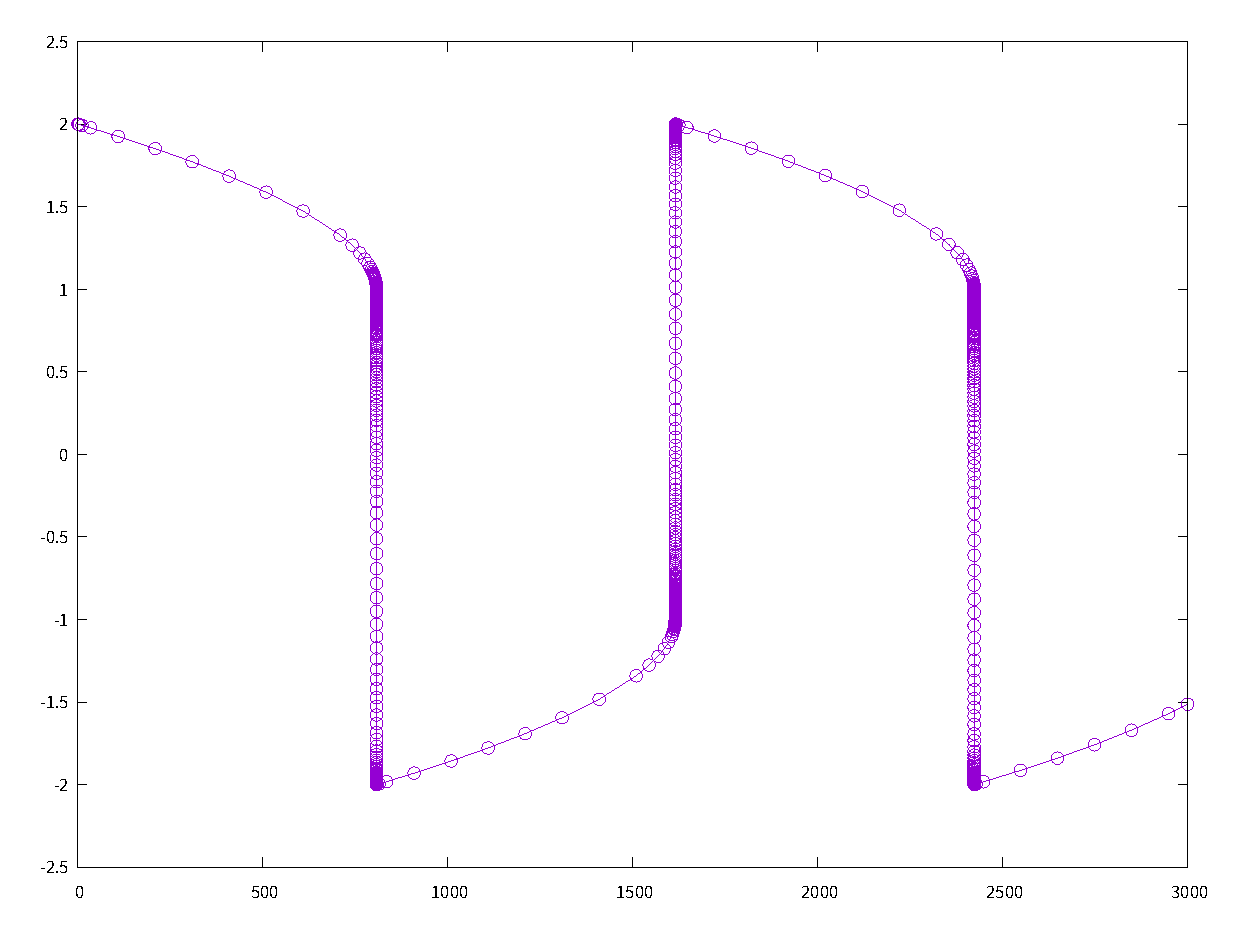
\includegraphics[width=0.95\linewidth]{figures/7-4.eps}
      \caption*{\small $s=1$,$n=918$}
  \end{minipage}
  \hspace{.31em}
  \begin{minipage}[t]{0.32\linewidth}
      \centering
      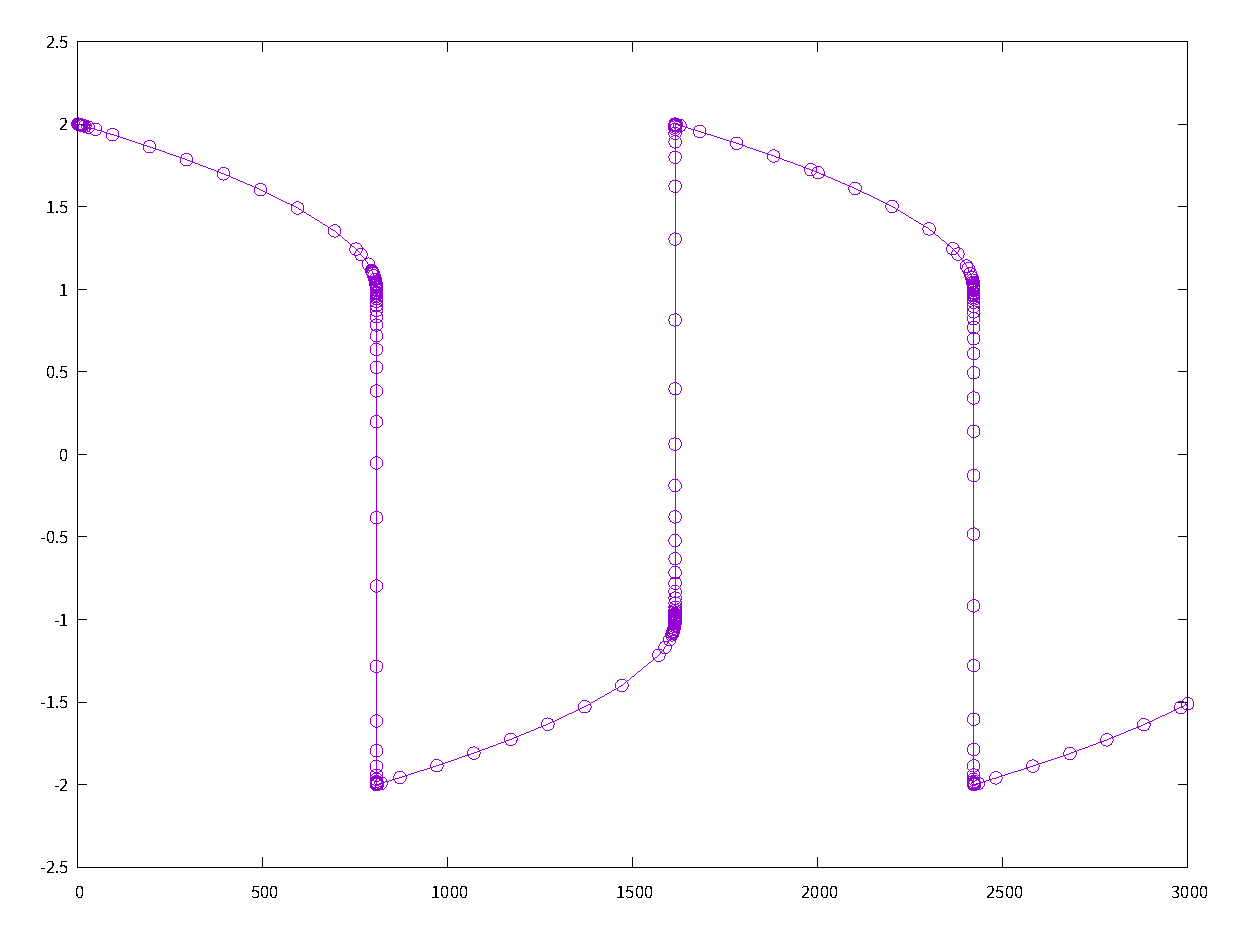
\includegraphics[width=0.95\linewidth]{figures/7-5.eps}
      \caption*{\small $s=2$,$n=269$}
  \end{minipage}
  \hspace{.31em}
  \begin{minipage}[t]{0.32\linewidth}
      \centering
      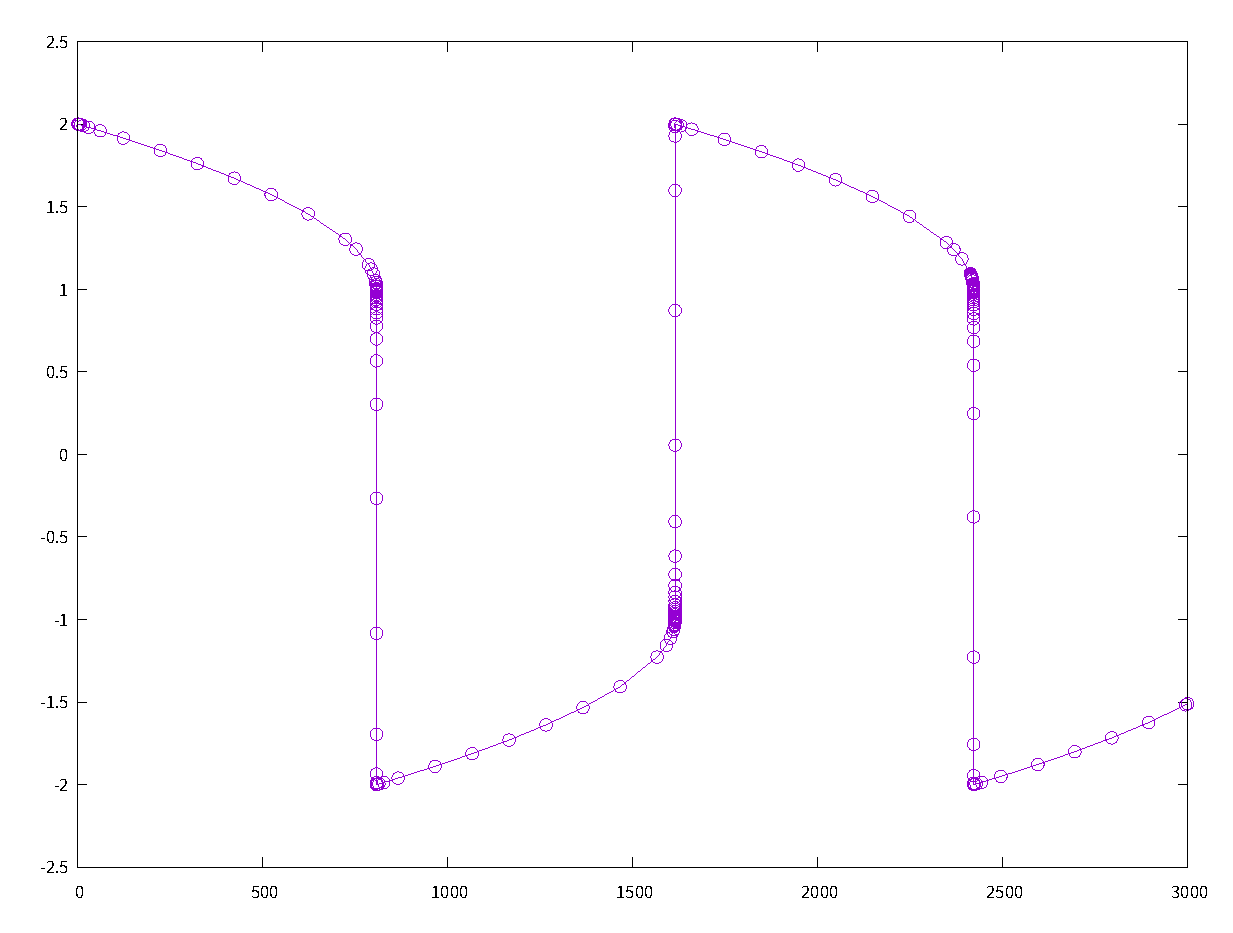
\includegraphics[width=0.95\linewidth]{figures/7-6.eps}
      \caption*{\small $s=3$,$n=207$}
  \end{minipage}
\end{figure}
\vspace{-.5em}

\subsection{结论}

在以非刚性方程为例的收敛性测试中,A-GLRK$s$方法表现出了$2s+1$阶的收敛率,这是因为采用了Richardson外插法作为一步误差估计,从而使得步长控制下的一步误差升了一阶。

与原始的GLRK方法对比,A-GLRK方法优势明显,但在非刚性方程上的表现不如DOPRI8方法。

A-GLRK方法的最大优势在于刚性方程的求解。此外,Dormand-Prince方法的Butcher表需要繁琐的人工计算,但A-GLRK方法的Butcher表可以自动计算,这让我们能轻松构造高阶自适应数值积分方法。

\section{自适应ESDIRK方法}

与A-GLRK一样,用Richardson外插法作为误差估计,来实现自适应ESDIRK.

\subsection{非刚性方程测试}

使用限制性三体问题轨道一测试A-ESDIRK方法,让Tolerance每次下降到原来的$\frac{1}{32}$,结果如下表。

\begin{table}[H]
  \centering
  \begin{tabular}{c|cccc|c}
    Tolerance$(\times 10^{-13})$ & 32768 & 1024 & 32 & 1 & 增长率 \\ \hline
    所需步数 & 671 & 1343  & 2686 & 5371 & 2.00   \\
    计算时间(s) & 0.0388 & 0.0615  & 0.112  & 0.212 & 
  \end{tabular}
\end{table}

设Tolerance为$5\times 10^{-5}$,绘制图像如下。

\begin{figure}[H]
  \centering
  \includegraphics[width=0.32\textwidth]{figures/8-1.eps}
  \caption*{A-ESDIRK,$n=104$}
\end{figure}

\subsection{刚性方程测试}

用Van der Pol方程测试A-ESDIRK对刚性方程的求解能力。在不同的Tolerance下,需要的步数与计算时间如下表。

\begin{table}[H]
  \centering
  \begin{tabular}{c|cccc}
    Tolerance & $10^{-4}$ & $10^{-6}$ & $10^{-8}$ & $10^{-10}$ \\ \hline
    所需步数 & 376 & 638 & 1273 & 3382   \\
    计算时间(s) & 0.375  & 0.296 & 0.161 & 0.254 
  \end{tabular}
\end{table}

注意到步数多时计算时间反而少,这与我们隐式方法的迭代实现有关(见2.2.1节)。步数少的时候,解的误差比较大,从而隐式方法的第一种迭代不收敛,不得不调用牛顿迭代求解器,后者的速度更慢。而步数多的时候,解的误差小,隐式方法的第一种迭代能够收敛。

将Tolerance为$10^{-4}$时的求解结果绘制图像如下。

\begin{figure}[H]
  \centering
  \includegraphics[width=0.32\textwidth]{figures/8-2.eps}
  \caption*{A-ESDIRK,$n=376$}
\end{figure}
\vspace{-1em}

\subsection{结论}

在非刚性方程的测试中,A-ESDIRK表现出了$5$阶收敛性,这是因为采用了Richardson外插法作为一步误差估计。它在限制性三体问题上的表现不如Dormand-Prince方法。

在Van der Pol方程的测试中,A-ESDIRK的表现比与它同阶的A-GLRK$2$更好,比更高阶的A-GLRK$3$更差,没有充分体现出具有L稳定性的优势。我们将在第10节进行一个补充测试。

\section{自适应Radau-IIA方法}

与A-GLRK一样,用Richardson外插法作为误差估计,来实现自适应Radau-IIA.

\subsection{非刚性方程测试}

使用限制性三体问题轨道一作为样例测试A-RIIARK方法,$s=2$时,让Tolerance每次下降到原来的$\frac{1}{16}$,结果如下表。

\vspace{-.5em}
\begin{table}[H]
  \centering
  \begin{tabular}{c|cccc|c}
    Tolerance$(\times 10^{-13})$ & 4096 & 256 & 16 & 1 & 增长率 \\ \hline
    所需步数 & 3483 & 6967  & 13934 & 27868 & 2.00   \\
    计算时间(s) & 0.0725 & 0.132  & 0.244  & 0.43 & 
  \end{tabular}
\end{table}
\vspace{-.5em}

$s=3$时,让Tolerance每次下降到原来的$\frac{1}{64}$,结果如下表。

\vspace{-.5em}
\begin{table}[H]
  \centering
  \begin{tabular}{c|cccc|c}
    Tolerance$(\times 10^{-13})$ & 32768 & 1024 & 32 & 1 & 增长率 \\ \hline
    所需步数 & 687 & 1374  & 2747 & 5495 & 2.00   \\
    计算时间(s) & 0.0203 & 0.0353 & 0.0629  & 0.102  & 
  \end{tabular}
\end{table}

将Tolerance设置到肉眼不可分辨,计算结果绘制图像如下。

\begin{figure}[H]
  \centering
  \begin{minipage}[t]{0.35\linewidth}
      \centering
      \includegraphics[width=0.95\linewidth]{figures/9-1.eps}
      \caption*{\small $s=2$,$\varepsilon=2\times 10^{-5}$,$n=221$}
  \end{minipage}
  \hspace{2em}
  \begin{minipage}[t]{0.35\linewidth}
      \centering
      \includegraphics[width=0.95\linewidth]{figures/9-2.eps}
      \caption*{\small $s=3$,$\varepsilon=10^{-4}$,$n=66$}
  \end{minipage}
\end{figure}

下面来测试A-RIIARK在长时间尺度下的求解准确性,将积分区间由$[0,T]$变为$[0,5T]$,取$s=4,5,6$,Tolerance设为$2\times 10^{-15}$,分别绘制轨道如下。

\begin{figure}[H]
  \centering
  \begin{minipage}[t]{0.32\linewidth}
      \centering
      \includegraphics[width=0.95\linewidth]{figures/9-3.eps}
      \caption*{\small $s=4$,$n=4190$,0.252秒}
  \end{minipage}
  \hspace{.31em}
  \begin{minipage}[t]{0.32\linewidth}
      \centering
      \includegraphics[width=0.95\linewidth]{figures/9-4.eps}
      \caption*{\small $s=5$,$n=2109$,0.227秒}
  \end{minipage}
  \hspace{.31em}
  \begin{minipage}[t]{0.32\linewidth}
      \centering
      \includegraphics[width=0.95\linewidth]{figures/9-5.eps}
      \caption*{\small $s=6$,$n=859$,0.216秒}
  \end{minipage}
\end{figure}
\vspace{-.5em}

当$s=6$时,轨道没有发生肉眼可见的偏离。

\vspace{-.5em}
\subsection{刚性方程测试}

用Van der Pol方程(1.2)测试A-RIIARK方法,在不同的Tolerance下求解,A-RIIARK$2$所需步数如下表。

\vspace{-.5em}
\begin{table}[H]
  \centering
  \begin{tabular}{c|cccc}
    Tolerance & $10^{-4}$ & $10^{-6}$ & $10^{-8}$ \\ \hline
    所需步数 & 421 & 1144 & 3776   \\
    计算时间(s) & 0.115  & 0.0491  & 0.111  
  \end{tabular}
\end{table}
\vspace{-.5em}

A-RIIARK$3$所需步数如下表。

\vspace{-.5em}
\begin{table}[H]
  \centering
  \begin{tabular}{c|cccc}
    Tolerance & $10^{-4}$ & $10^{-6}$ & $10^{-8}$ \\ \hline
    所需步数 & 200 & 322 & 642   \\
    计算时间(s) & 0.283  & 0.112  & 0.0944  
  \end{tabular}
\end{table}
\vspace{-.5em}

将Tolerance取$10^{-4}$时的计算结果绘制图像如下(我们限制了步长最大为300)。

\vspace{-.5em}
\begin{figure}[H]
  \centering
  \begin{minipage}[t]{0.32\linewidth}
      \centering
      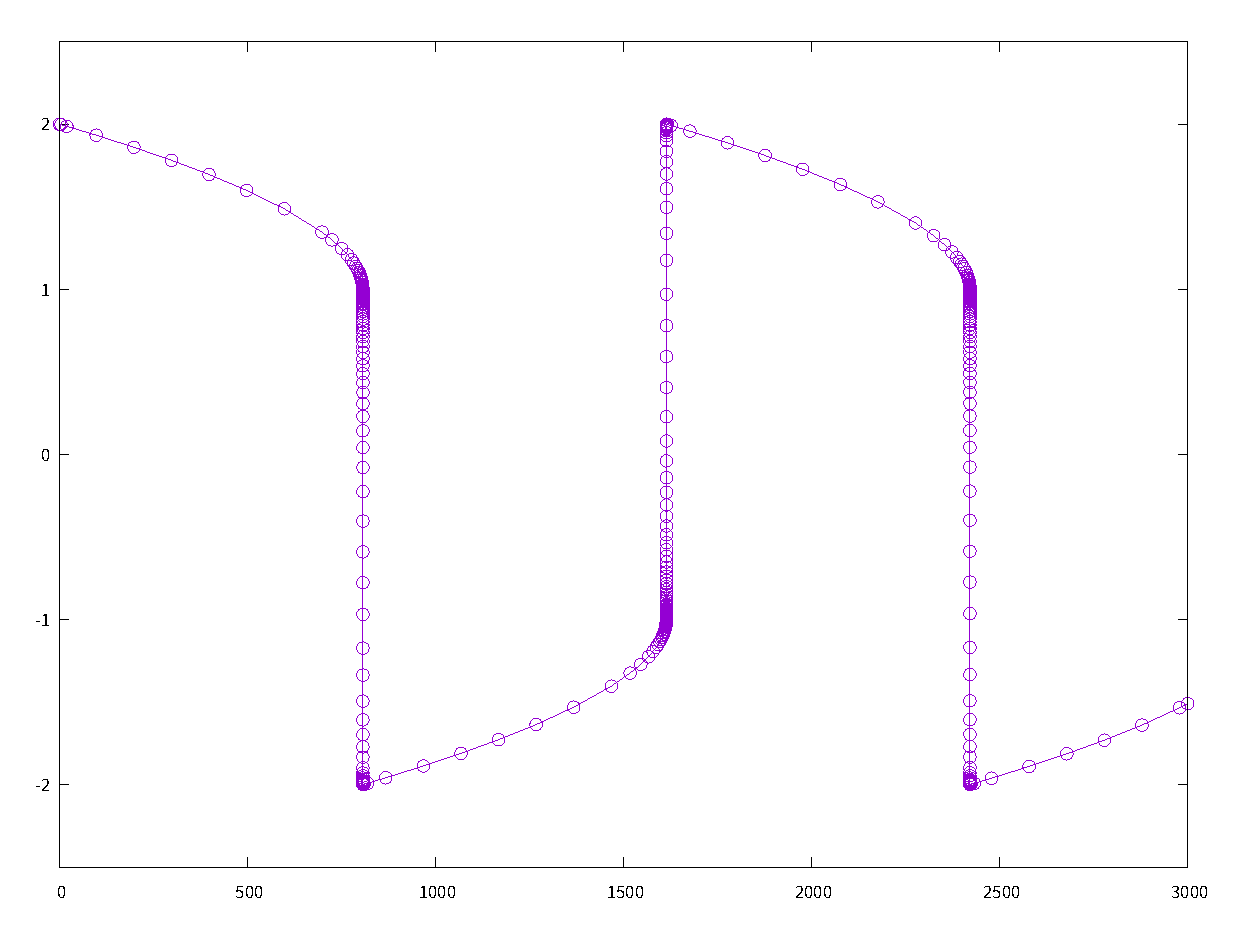
\includegraphics[width=0.95\linewidth]{figures/9-6.eps}
      \caption*{\small $s=2$,$n=421$}
  \end{minipage}
  \hspace{.31em}
  \begin{minipage}[t]{0.32\linewidth}
      \centering
      \includegraphics[width=0.95\linewidth]{figures/9-7.eps}
      \caption*{\small $s=3$,$n=200$}
  \end{minipage}
  \hspace{.31em}
  \begin{minipage}[t]{0.32\linewidth}
      \centering
      \includegraphics[width=0.95\linewidth]{figures/9-8.eps}
      \caption*{\small $s=4$,$n=170$}
  \end{minipage}
\end{figure}
\vspace{-.5em}

\subsection{结论}

在以非刚性方程为例的收敛性测试中,A-RIIARK$s$方法表现出了$2s$阶的收敛率,这是因为采用了Richardson外插法作为一步误差估计,从而使得步长控制下的一步误差升了一阶。

与原始的RIIARK方法对比,A-RIIARK方法优势明显,高阶的A-RIIARK在长时间尺度下的稳定度很好,但在非刚性方程上的求解速度不如DOPRI8方法。

A-RIIARK最大的优势在于刚性方程的求解,它在刚性方程上的求解无论是速度还是效果都比A-ESDIRK与A-GLRK要好。下面这个例子将更好地反映这个问题。

\vspace{-1em}
\section{对比测试:隐式自适应方法的刚性稳定性}

\vspace{-.5em}
前文的Van der Pol方程测试并没有显示出L稳定性的作用,因此我们做一组补充测试,目的是凸显L稳定性的重要性。考虑讲义Example 11.144中的方程:
\begin{equation}
  u'(t)=\lambda(u-\cos t)-\sin t,\quad u(0)=\eta.
\end{equation}

方程的真解为:
\begin{equation}
  u(t)=e^{\lambda t}(\eta-1)+\cos t.
\end{equation}

我们取$\lambda=-10^6,\eta=1.5$,则它在很短的时间内迅速收敛至余弦曲线,如下图。

\vspace{-.5em}
\begin{figure}[H]
  \centering
  \includegraphics[width=0.3\textwidth]{figures/10-1.eps}
\end{figure}
\vspace{-.5em}

为了方便测试,我们将这个方程也加入了内置函数库。将\verb|"Problem"|参数设为\verb|"Stiff Sample Problem"|即可直接使用。在$[0,3]$中求解这个方程,在不同的Tolerance下,各种隐式自适应方法所需步数与时间如下表。

\vspace{-.3em}
\begin{table}[H]
  \centering
  \begin{tabular}{c|cccc}
    Tolerance & $10^{-8}$ & $10^{-10}$ & $10^{-12}$ & $10^{-13}$ \\ \hline
    A-GLRK$3$ & 109步,0.372秒\;\;\;\; & 367步,1.36秒\;\;\;\; & 807步,2.92秒\;\;\;\; & 1410步,5.46秒 \\
    A-RIIARK$3$ & 43步,0.0886秒\;\;\;\; & 91步,0.134秒\;\;\;\; & 227步,0.388秒\;\;\;\; & 383步,0.769秒 \\
    A-ESDIRK & 64步,0.0382秒\;\;\;\; & 193步,0.136秒\;\;\;\; & 948步,1.16秒\;\;\;\; & 2497步,3.7秒
  \end{tabular}
\end{table}
\vspace{-.8em}

注意,上面三种方法的阶数分别为$7,6,5$(因为Richardson外插法的缘故,可以认为比原始方法高一阶)。但是作为最高阶的A-GLRK$3$,在这个方程上居然表现最差,这足以说明L稳定性的重要性。

事实上,图像能更好地说明问题。将三种方法在Tolerance为$10^{-8}$时的解绘制如下。我们发现,所有方法在一开始取的点都很密集,但具有L稳定性的方法在收敛至余弦曲线后迅速增大步长完成计算,不具有L稳定性的方法则因为解的振荡而无法增大步长。

\begin{figure}[H]
  \centering
  \begin{minipage}[t]{0.32\linewidth}
      \centering
      \includegraphics[width=0.95\linewidth]{figures/10-2.eps}
      \caption*{\small A-GLRK$3$,$n=109$}
  \end{minipage}
  \hspace{.31em}
  \begin{minipage}[t]{0.32\linewidth}
      \centering
      \includegraphics[width=0.95\linewidth]{figures/10-3.eps}
      \caption*{\small A-RIIARK$3$,$n=43$}
  \end{minipage}
  \hspace{.31em}
  \begin{minipage}[t]{0.32\linewidth}
      \centering
      \includegraphics[width=0.95\linewidth]{figures/10-4.eps}
      \caption*{\small A-ESDIRK,$n=64$}
  \end{minipage}
\end{figure}

\section{Adams-Bashforth方法}

\subsection{初值的敏感性及稳定的计算方法}

在限制性三体问题的轨道一中,卫星的起始位置与月球的距离很近,因此受月球引力影响很大,初值稍有一点偏差就会对整个求解过程产生严重的影响。我们现在使用AB$3$求解器,步数设为$50000$,前两个初值分别采用向前欧拉法、高阶的RK方法计算,结果如下图。

\begin{figure}[H]
  \centering
  \begin{minipage}[t]{0.35\linewidth}
      \centering
      \includegraphics[width=0.95\linewidth]{figures/11-1.eps}
      \caption*{\small 前两个初值由向前欧拉法计算}
  \end{minipage}
  \hspace{2em}
  \begin{minipage}[t]{0.35\linewidth}
      \centering
      \includegraphics[width=0.95\linewidth]{figures/11-2.eps}
      \caption*{\small 前两个初值由RIIARK$2$法计算}
  \end{minipage}
\end{figure}

仅仅是开头的两个初值就对结果产生了如此巨大的影响。因此我们必须采用非常精确的方法计算初值,最好用阶数不低于$p$的方法。在我们的求解器中,一个$p$阶LMM方法的前面几个初值,将用$\left\lceil\frac{p}{2}\right\rceil$阶段的Radau-IIA方法计算。这样可以保证$p$能取得任意大,也通过Radau-IIA的L稳定性保证了初值的稳定性。

\subsection{收敛性测试}

仍以限制性三体问题做测试。我们使用AB$p$方法,令步长为$\frac{T}{n}$,取不同的$n$,对轨道一测试,将$T$时刻的数值解与初始值比较。$p=1$结果如下。

\vspace{-.5em}
\begin{table}[H]
  \centering
  \renewcommand\arraystretch{0.85}
  \begin{tabular}{cc|ccc|c}
  \multicolumn{2}{c|}{$n\;(\times 10^7)$}                  & 2 & 4 & 8  & 收敛阶 \\ \hline
  \multicolumn{1}{c|}{\multirow{4}{*}{$T$时刻误差}} & \multicolumn{1}{c|}{$u_1$} &  0.000583002  &  0.000517543  & 0.000338637    &  0.61   \\
  \multicolumn{1}{c|}{}                         & \multicolumn{1}{c|}{$u_2$} &   0.00617976    & 0.00321683  & 0.001636    &  0.98   \\
  \multicolumn{1}{c|}{}                         & \multicolumn{1}{c|}{$u_4$} &   0.609395    & 0.410059  & 0.236732     &  0.79   \\
  \multicolumn{1}{c|}{}                         & \multicolumn{1}{c|}{$u_5$} &   0.457729    & 0.214632  & 0.093224     &  1.20  \\ \hline
  \multicolumn{2}{c|}{求解时间(s)} & 17.6 & 33.2 & 69.1 & 
  \end{tabular}
\end{table}
\vspace{-.8em}

由于误差太大,收敛阶的估计不可靠。要想得到准确的收敛阶,需要测试更小的步长,但我们的计算机运算能力有限,因此我们放弃这项测试。$p=2$结果如下。

\vspace{-.5em}
\begin{table}[H]
  \centering
  \renewcommand\arraystretch{0.85}
  \begin{tabular}{cc|ccc|c}
  \multicolumn{2}{c|}{$n\;(\times 10^6)$}                  & 2.5 & 5 & 10  & 收敛阶 \\ \hline
  \multicolumn{1}{c|}{\multirow{4}{*}{$T$时刻误差}} & \multicolumn{1}{c|}{$u_1$} &  5.37843e-05  &  1.32132e-05  & 3.28959e-06    &  2.01   \\
  \multicolumn{1}{c|}{}                         & \multicolumn{1}{c|}{$u_2$} &   0.000181596    & 4.54249e-05  & 1.13601e-05    &  2.00   \\
  \multicolumn{1}{c|}{}                         & \multicolumn{1}{c|}{$u_4$} &   0.0298535    & 0.00740036  & 0.00184648     &  2.00   \\
  \multicolumn{1}{c|}{}                         & \multicolumn{1}{c|}{$u_5$} &   0.00778674   & 0.00202049  & 0.000509764     &  1.99  \\ \hline
  \multicolumn{2}{c|}{求解时间(s)} & 2.05 & 3.93 & 8.01 & 
  \end{tabular}
\end{table}
\vspace{-.8em}

$p=3$结果如下。

\vspace{-.5em}
\begin{table}[H]
  \centering
  \renewcommand\arraystretch{0.85}
  \begin{tabular}{cc|ccc|c}
  \multicolumn{2}{c|}{$n\;(\times 10^6)$}                  & 1 & 2 & 4  & 收敛阶 \\ \hline
  \multicolumn{1}{c|}{\multirow{4}{*}{$T$时刻误差}} & \multicolumn{1}{c|}{$u_1$} &  8.70394e-07  &  1.11301e-07  & 1.4072e-08    &  2.98   \\
  \multicolumn{1}{c|}{}                         & \multicolumn{1}{c|}{$u_2$} &   3.07092e-06    & 3.921e-07  & 4.9531e-08    &  2.98   \\
  \multicolumn{1}{c|}{}                         & \multicolumn{1}{c|}{$u_4$} &   0.000498694    & 6.36659e-05  & 8.04244e-06     &  2.98   \\
  \multicolumn{1}{c|}{}                         & \multicolumn{1}{c|}{$u_5$} &   0.0001352   & 1.73071e-05  & 2.18848e-06     &  2.98  \\ \hline
  \multicolumn{2}{c|}{求解时间(s)} & 0.791 & 1.71 & 3.16 & 
  \end{tabular}
\end{table}
\vspace{-.8em}

$p=4$结果如下。

\vspace{-.5em}
\begin{table}[H]
  \centering
  \renewcommand\arraystretch{0.8}
  \begin{tabular}{cc|ccc|c}
  \multicolumn{2}{c|}{$n\;(\times 10^6)$}                  & 0.5 & 1 & 2  & 收敛阶 \\ \hline
  \multicolumn{1}{c|}{\multirow{4}{*}{$T$时刻误差}} & \multicolumn{1}{c|}{$u_1$} &  8.05461e-07  &  5.10134e-08  & 3.20246e-09    &  3.99   \\
  \multicolumn{1}{c|}{}                         & \multicolumn{1}{c|}{$u_2$} &   2.70583e-06    & 1.71126e-07  & 1.0739e-08    &  3.99   \\
  \multicolumn{1}{c|}{}                         & \multicolumn{1}{c|}{$u_4$} &   0.000439774    & 2.78186e-05  & 1.7458e-06     &  3.99   \\
  \multicolumn{1}{c|}{}                         & \multicolumn{1}{c|}{$u_5$} &   0.000125495   & 7.94058e-06  & 4.98454e-07     &  3.99  \\ \hline
  \multicolumn{2}{c|}{求解时间(s)} & 0.414 & 0.821 & 1.85 & 
  \end{tabular}
\end{table}
\vspace{-.8em}

各方法的步数分别取$4000000,400000,50000,50000$绘图如下。

\vspace{-.5em}
\begin{figure}[H]
  \centering
  \begin{minipage}[t]{0.35\linewidth}
      \centering
      \includegraphics[width=0.95\linewidth]{figures/11-3.eps}
      \caption*{\small $p=1,n=4000000$}
  \end{minipage}
  \hspace{2em}
  \begin{minipage}[t]{0.35\linewidth}
      \centering
      \includegraphics[width=0.95\linewidth]{figures/11-4.eps}
      \caption*{\small $p=2,n=400000$}
  \end{minipage}
  \begin{minipage}[t]{0.35\linewidth}
    \centering
    \includegraphics[width=0.95\linewidth]{figures/11-5.eps}
    \caption*{\small $p=3,n=50000$}
\end{minipage}
\hspace{2em}
\begin{minipage}[t]{0.35\linewidth}
    \centering
    \includegraphics[width=0.95\linewidth]{figures/11-6.eps}
    \caption*{\small $p=4,n=50000$}
\end{minipage}
\end{figure}
\vspace{-1em}

对轨道二测试,这里的收敛阶用Richardson外插法估计,$p=1$时结果如下。

\vspace{-.5em}
\begin{table}[H]
  \centering
  \renewcommand\arraystretch{0.8}
  \begin{tabular}{cc|ccc|c}
  \multicolumn{2}{c|}{$n\;(\times 10^7)$}                  & 0.5 & 1 & 2  & 收敛阶 \\ \hline
  \multicolumn{1}{c|}{\multirow{4}{*}{\makecell{与$2n$步的解\\在$T$时刻的误差}}} & \multicolumn{1}{c|}{$u_1$} &  0.0055131  &  0.00264892  & 0.00129961    &  1.03   \\
  \multicolumn{1}{c|}{}                         & \multicolumn{1}{c|}{$u_2$} &   0.00521829    & 0.00259169  & 0.00129085    &  1.00   \\
  \multicolumn{1}{c|}{}                         & \multicolumn{1}{c|}{$u_4$} &   0.0254778    & 0.0117395  & 0.00564074     &  1.04   \\
  \multicolumn{1}{c|}{}                         & \multicolumn{1}{c|}{$u_5$} &   0.00988692   & 0.00512506  & 0.00259232     &  0.99  \\ \hline
  \multicolumn{2}{c|}{求解时间(s)} & 3.53 & 7.18 & 15.5 & 
  \end{tabular}
\end{table}
\vspace{-.8em}

$p=2$时结果如下。

\vspace{-.5em}
\begin{table}[H]
  \centering
  \renewcommand\arraystretch{0.8}
  \begin{tabular}{cc|ccc|c}
  \multicolumn{2}{c|}{$n\;(\times 10^6)$}                  & 0.5 & 1 & 2  & 收敛阶 \\ \hline
  \multicolumn{1}{c|}{\multirow{4}{*}{\makecell{与$2n$步的解\\在$T$时刻的误差}}} & \multicolumn{1}{c|}{$u_1$} &  4.65551e-07  &  1.16958e-07  & 2.93113e-08    &  2.00   \\
  \multicolumn{1}{c|}{}                         & \multicolumn{1}{c|}{$u_2$} &   1.38301e-07    & 3.40018e-08  & 8.42821e-09    &  2.01   \\
  \multicolumn{1}{c|}{}                         & \multicolumn{1}{c|}{$u_4$} &   2.10322e-06    & 5.28232e-07  & 1.32365e-07     &  2.00   \\
  \multicolumn{1}{c|}{}                         & \multicolumn{1}{c|}{$u_5$} &   8.47832e-07   & 2.13122e-07  & 5.34268e-08     &  2.00  \\ \hline
  \multicolumn{2}{c|}{求解时间(s)} & 0.344 & 0.672 & 1.51 & 
  \end{tabular}
\end{table}
\vspace{-.8em}

$p=3$时结果如下。

\vspace{-.5em}
\begin{table}[H]
  \centering
  \renewcommand\arraystretch{0.8}
  \begin{tabular}{cc|ccc|c}
  \multicolumn{2}{c|}{$n\;(\times 10^5)$}                  & 1 & 2 & 4  & 收敛阶 \\ \hline
  \multicolumn{1}{c|}{\multirow{4}{*}{\makecell{与$2n$步的解\\在$T$时刻的误差}}} & \multicolumn{1}{c|}{$u_1$} &  8.54799e-07  &  1.06845e-07  & 1.33545e-08    &  3.00   \\
  \multicolumn{1}{c|}{}                         & \multicolumn{1}{c|}{$u_2$} &   8.60002e-07    & 1.07502e-07  & 1.34368e-08    &  3.00   \\
  \multicolumn{1}{c|}{}                         & \multicolumn{1}{c|}{$u_4$} &   3.63951e-06    & 4.54921e-07  & 5.686e-08     &  3.00   \\
  \multicolumn{1}{c|}{}                         & \multicolumn{1}{c|}{$u_5$} &   1.74518e-06   & 2.18139e-07  & 2.72648e-08     &  3.00  \\ \hline
  \multicolumn{2}{c|}{求解时间(s)} & 0.0894 & 0.182 & 0.339 & 
  \end{tabular}
\end{table}
\vspace{-.8em}

$p=4$时结果如下(这里收敛阶超过了4)。

\vspace{-.5em}
\begin{table}[H]
  \centering
  \renewcommand\arraystretch{0.8}
  \begin{tabular}{cc|ccc|c}
  \multicolumn{2}{c|}{$n\;(\times 10^4)$}                  & 0.5 & 1 & 2  & 收敛阶 \\ \hline
  \multicolumn{1}{c|}{\multirow{4}{*}{\makecell{与$2n$步的解\\在$T$时刻的误差}}} & \multicolumn{1}{c|}{$u_1$} &  2.38152e-05  &  3.94598e-07  & 9.64539e-09    &  5.28   \\
  \multicolumn{1}{c|}{}                         & \multicolumn{1}{c|}{$u_2$} &   3.77951e-05    & 1.26833e-06  & 4.49022e-08    &  4.82   \\
  \multicolumn{1}{c|}{}                         & \multicolumn{1}{c|}{$u_4$} &   9.90411e-05    & 1.51898e-06  & 5.15866e-08     &  4.78   \\
  \multicolumn{1}{c|}{}                         & \multicolumn{1}{c|}{$u_5$} &   5.06315e-05   & 9.44781e-07  & 1.05412e-08     &  6.45  \\ \hline
  \multicolumn{2}{c|}{求解时间(s)} & 0.0894 & 0.011 & 0.0222 & 
  \end{tabular}
\end{table}
\vspace{-.8em}

各方法的步数分别取$5000000,10000,8000,2500$绘图如下。

\begin{figure}[H]
  \centering
  \begin{minipage}[t]{0.35\linewidth}
      \centering
      \includegraphics[width=0.95\linewidth]{figures/11-7.eps}
      \caption*{\small $p=1,n=5000000$}
  \end{minipage}
  \hspace{2em}
  \begin{minipage}[t]{0.35\linewidth}
      \centering
      \includegraphics[width=0.95\linewidth]{figures/11-8.eps}
      \caption*{\small $p=2,n=10000$}
  \end{minipage}
  \begin{minipage}[t]{0.35\linewidth}
    \centering
    \includegraphics[width=0.95\linewidth]{figures/11-9.eps}
    \caption*{\small $p=3,n=8000$}
\end{minipage}
\hspace{2em}
\begin{minipage}[t]{0.35\linewidth}
    \centering
    \includegraphics[width=0.95\linewidth]{figures/11-10.eps}
    \caption*{\small $p=4,n=2500$}
\end{minipage}
\end{figure}

\subsection{结论}

轨道一$p=1$、轨道二$p=4$的数值测试在收敛阶上出现问题。

AB$p$方法具有$p$阶的累积误差,是$p$阶精度的方法,且初值敏感。

\vspace{-1.3em}
\section{Adams-Moulton方法}

\subsection{隐式LMM的计算方法}

与隐式RK一样,我们提出两种计算方法。下面是\textbf{第一种计算方法}。

\begin{enumerate}[itemindent=1em]
  \item $\mathbf{U}^{n+s}\gets \mathbf{U}^{n+s-1}$.
  \item $\hat{\mathbf{U}}^{n+s}\gets \mathbf{U}^{n+s}$,$\mathbf{U}^{n+s}\gets \mathbf{U}^{n+s-1}+k\sum\limits_{j=1}^s\beta_j\mathbf{f}(\mathbf{U}^{n+j},t_{n+j})$.
  \item 若$||\hat{\mathbf{U}}^{n+s}-\mathbf{U}^{n+s}|| < \varepsilon$,结束,否则返回步骤2.
\end{enumerate}

第二种计算方法就是牛顿迭代法。当第一种方法计算40次不收敛时,就用牛顿迭代法求解。

\subsection{收敛性测试}

仍以限制性三体问题做测试。我们使用AM$p$方法,令步长为$\frac{T}{n}$,取不同的$n$,对轨道一测试,将$T$时刻的数值解与初始值比较。$p=2$结果如下。

\vspace{-.5em}
\begin{table}[H]
  \centering
  \renewcommand\arraystretch{0.8}
  \begin{tabular}{cc|ccc|c}
  \multicolumn{2}{c|}{$n\;(\times 10^6)$}                  & 1 & 2 & 4  & 收敛阶 \\ \hline
  \multicolumn{1}{c|}{\multirow{4}{*}{$T$时刻误差}} & \multicolumn{1}{c|}{$u_1$} &  6.37208e-05  &  1.6304e-05  & 4.0996e-06    &  1.99   \\
  \multicolumn{1}{c|}{}                         & \multicolumn{1}{c|}{$u_2$} &   0.000227146    & 5.68145e-05  & 1.42051e-05    &  2.00   \\
  \multicolumn{1}{c|}{}                         & \multicolumn{1}{c|}{$u_4$} &   0.0363206    & 0.00919204  & 0.00230492     &  2.00   \\
  \multicolumn{1}{c|}{}                         & \multicolumn{1}{c|}{$u_5$} &   0.0107967    & 0.00259356  & 0.000641599     &  2.02  \\ \hline
  \multicolumn{2}{c|}{求解时间(s)} & 1.47 & 3.22 & 5.66 & 
  \end{tabular}
\end{table}
\vspace{-.8em}

$p=3$结果如下。

\vspace{-.5em}
\begin{table}[H]
  \centering
  \renewcommand\arraystretch{0.8}
  \begin{tabular}{cc|ccc|c}
  \multicolumn{2}{c|}{$n\;(\times 10^5)$}                  & 4 & 8 & 16  & 收敛阶 \\ \hline
  \multicolumn{1}{c|}{\multirow{4}{*}{$T$时刻误差}} & \multicolumn{1}{c|}{$u_1$} &  1.45118e-06  &  1.89548e-07  & 2.42012e-08    &  2.97   \\
  \multicolumn{1}{c|}{}                         & \multicolumn{1}{c|}{$u_2$} &   5.13822e-06    & 6.68618e-07  & 8.52349e-08    &  2.97   \\
  \multicolumn{1}{c|}{}                         & \multicolumn{1}{c|}{$u_4$} &   0.000833905    & 0.000108554  & 1.38394e-05     &  2.97   \\
  \multicolumn{1}{c|}{}                         & \multicolumn{1}{c|}{$u_5$} &   0.000226146   & 2.94864e-05  & 3.76396e-06     &  2.97  \\ \hline
  \multicolumn{2}{c|}{求解时间(s)} & 0.676 & 1.34 & 2.39 & 
  \end{tabular}
\end{table}
\vspace{-.8em}

$p=4$结果如下。

\vspace{-.5em}
\begin{table}[H]
  \centering
  \renewcommand\arraystretch{0.8}
  \begin{tabular}{cc|ccc|c}
  \multicolumn{2}{c|}{$n\;(\times 10^5)$}                  & 2 & 4 & 8  & 收敛阶 \\ \hline
  \multicolumn{1}{c|}{\multirow{4}{*}{$T$时刻误差}} & \multicolumn{1}{c|}{$u_1$} &  2.33539e-06  &  1.49452e-07  & 9.44687e-09    &  3.98   \\
  \multicolumn{1}{c|}{}                         & \multicolumn{1}{c|}{$u_2$} &   7.84982e-06    & 5.01761e-07  & 3.16867e-08    &  3.99   \\
  \multicolumn{1}{c|}{}                         & \multicolumn{1}{c|}{$u_4$} &   0.00127668    & 8.1569e-05  & 5.15114e-06     &  3.99   \\
  \multicolumn{1}{c|}{}                         & \multicolumn{1}{c|}{$u_5$} &   0.000362429   & 2.32574e-05  & 1.47036e-06     &  3.98  \\ \hline
  \multicolumn{2}{c|}{求解时间(s)} & 0.38 & 0.711 & 1.49 & 
  \end{tabular}
\end{table}
\vspace{-.8em}

$p=5$结果如下(这里收敛阶超过了5)。

\vspace{-.5em}
\begin{table}[H]
  \centering
  \renewcommand\arraystretch{0.8}
  \begin{tabular}{cc|ccc|c}
  \multicolumn{2}{c|}{$n\;(\times 10^5)$}                  & 1 & 2 & 4  & 收敛阶 \\ \hline
  \multicolumn{1}{c|}{\multirow{4}{*}{$T$时刻误差}} & \multicolumn{1}{c|}{$u_1$} &  1.44067e-06  &  2.5908e-08  & 4.67902e-10    &  5.79   \\
  \multicolumn{1}{c|}{}                         & \multicolumn{1}{c|}{$u_2$} &   4.54827e-06    & 7.79218e-08  & 1.29963e-09    &  5.90   \\
  \multicolumn{1}{c|}{}                         & \multicolumn{1}{c|}{$u_4$} &   0.000740406    & 1.27065e-05  & 2.12444e-07     & 5.90   \\
  \multicolumn{1}{c|}{}                         & \multicolumn{1}{c|}{$u_5$} &   0.000224524   & 4.03229e-06  & 7.28449e-08     & 5.79  \\ \hline
  \multicolumn{2}{c|}{求解时间(s)} & 0.203 & 0.383 & 0.741 & 
  \end{tabular}
\end{table}
\vspace{-.8em}

各方法的步数分别取$100000,40000,40000,10000$绘图如下。

\vspace{-.5em}
\begin{figure}[H]
  \centering
  \begin{minipage}[t]{0.35\linewidth}
      \centering
      \includegraphics[width=0.95\linewidth]{figures/12-1.eps}
      \caption*{\small $p=2,n=100000$}
  \end{minipage}
  \hspace{2em}
  \begin{minipage}[t]{0.35\linewidth}
      \centering
      \includegraphics[width=0.95\linewidth]{figures/12-2.eps}
      \caption*{\small $p=2,n=40000$}
  \end{minipage}
  \begin{minipage}[t]{0.35\linewidth}
    \centering
    \includegraphics[width=0.95\linewidth]{figures/12-3.eps}
    \caption*{\small $p=3,n=40000$}
  \end{minipage}
  \hspace{2em}
  \begin{minipage}[t]{0.35\linewidth}
      \centering
      \includegraphics[width=0.95\linewidth]{figures/12-4.eps}
      \caption*{\small $p=4,n=10000$}
  \end{minipage}
\end{figure}
\vspace{-1em}

对轨道二测试,这里的收敛阶用Richardson外插法估计,$p=2$时结果如下。

\vspace{-.8em}
\begin{table}[H]
  \centering
  \renewcommand\arraystretch{0.75}
  \begin{tabular}{cc|ccc|c}
  \multicolumn{2}{c|}{$n\;(\times 10^5)$}                  & 2.5 & 5 & 10  & 收敛阶 \\ \hline
  \multicolumn{1}{c|}{\multirow{4}{*}{\makecell{与$2n$步的解\\在$T$时刻的误差}}} & \multicolumn{1}{c|}{$u_1$} &  3.76097e-07  &  1.25347e-07  & 2.35032e-08    &  2.00   \\
  \multicolumn{1}{c|}{}                         & \multicolumn{1}{c|}{$u_2$} &   1.06961e-07    & 3.56562e-08  & 6.68756e-09    &  2.00   \\
  \multicolumn{1}{c|}{}                         & \multicolumn{1}{c|}{$u_4$} &   1.69816e-06    & 5.65966e-07  & 1.06122e-07     &  2.00   \\
  \multicolumn{1}{c|}{}                         & \multicolumn{1}{c|}{$u_5$} &   6.85727e-07   & 2.28541e-07  & 4.28523e-08     &  2.00  \\ \hline
  \multicolumn{2}{c|}{求解时间(s)} & 0.405 & 0.819 & 1.63 & 
  \end{tabular}
\end{table}
\vspace{-1em}

$p=3$时结果如下。

\vspace{-.8em}
\begin{table}[H]
  \centering
  \renewcommand\arraystretch{0.75}
  \begin{tabular}{cc|ccc|c}
  \multicolumn{2}{c|}{$n\;(\times 10^5)$}                  & 0.5 & 1 & 2  & 收敛阶 \\ \hline
  \multicolumn{1}{c|}{\multirow{4}{*}{\makecell{与$2n$步的解\\在$T$时刻的误差}}} & \multicolumn{1}{c|}{$u_1$} &  7.59808e-07  &  1.08523e-07  & 1.18698e-08    &  3.00   \\
  \multicolumn{1}{c|}{}                         & \multicolumn{1}{c|}{$u_2$} &   7.64456e-07    & 1.09208e-07  & 1.19432e-08    &  3.00   \\
  \multicolumn{1}{c|}{}                         & \multicolumn{1}{c|}{$u_4$} &   3.2351e-06    & 4.62059e-07  & 5.05387e-08     &  3.00   \\
  \multicolumn{1}{c|}{}                         & \multicolumn{1}{c|}{$u_5$} &   1.55123e-06   & 2.21566e-07  & 2.42339e-08     &  3.00  \\ \hline
  \multicolumn{2}{c|}{求解时间(s)} & 0.112 & 0.193 & 0.368 & 
  \end{tabular}
\end{table}
\vspace{-1em}

$p=4$时结果如下(这里出于未知原因收敛阶不对,增大、减小$n$均不对)。

\vspace{-.8em}
\begin{table}[H]
  \centering
  \renewcommand\arraystretch{0.75}
  \begin{tabular}{cc|ccc|c}
  \multicolumn{2}{c|}{$n\;(\times 10^3)$}                  & 3 & 6 & 12  & 收敛阶 \\ \hline
  \multicolumn{1}{c|}{\multirow{4}{*}{\makecell{与$2n$步的解\\在$T$时刻的误差}}} & \multicolumn{1}{c|}{$u_1$} &  1.07968e-05  &  1.32633e-07  & 8.69294e-09    &  3.73   \\
  \multicolumn{1}{c|}{}                         & \multicolumn{1}{c|}{$u_2$} &   1.89588e-05    & 6.42769e-07  & 2.31584e-08    &  4.79   \\
  \multicolumn{1}{c|}{}                         & \multicolumn{1}{c|}{$u_4$} &   4.45645e-05    & 4.69373e-07  & 4.31946e-08     &  3.15   \\
  \multicolumn{1}{c|}{}                         & \multicolumn{1}{c|}{$u_5$} &   2.3239e-05   & 3.53269e-07  & 1.2365e-08     &  4.73  \\ \hline
  \multicolumn{2}{c|}{求解时间(s)} & 0.0109 & 0.0177 & 0.034 & 
  \end{tabular}
\end{table}
\vspace{-1em}

$p=5$时结果如下(这里出于未知原因收敛阶又对回来了……)。

\vspace{-.8em}
\begin{table}[H]
  \centering
  \renewcommand\arraystretch{0.75}
  \begin{tabular}{cc|ccc|c}
  \multicolumn{2}{c|}{$n\;(\times 10^3)$}                  & 3 & 6 & 12  & 收敛阶 \\ \hline
  \multicolumn{1}{c|}{\multirow{4}{*}{\makecell{与$2n$步的解\\在$T$时刻的误差}}} & \multicolumn{1}{c|}{$u_1$} &  1.54218e-05  &  4.86839e-07  & 1.52429e-08    &  5.00   \\
  \multicolumn{1}{c|}{}                         & \multicolumn{1}{c|}{$u_2$} &   1.53823e-05    & 4.87139e-07  & 1.52768e-08    &  4.99   \\
  \multicolumn{1}{c|}{}                         & \multicolumn{1}{c|}{$u_4$} &   6.58658e-05    & 2.07919e-06  & 6.50954e-08     &  5.00   \\
  \multicolumn{1}{c|}{}                         & \multicolumn{1}{c|}{$u_5$} &   3.12816e-05    & 9.87611e-07  & 3.09256e-08     &  5.00  \\ \hline
  \multicolumn{2}{c|}{求解时间(s)} & 0.0105 & 0.0152 & 0.0373 & 
  \end{tabular}
\end{table}
\vspace{-1em}

各方法的步数分别取$5000,4000,1200,1100$绘图如下。

\vspace{-1em}
\begin{figure}[H]
  \centering
  \begin{minipage}[t]{0.32\linewidth}
      \centering
      \includegraphics[width=0.95\linewidth]{figures/12-5.eps}
      \caption*{\small $p=2,n=5000$}
  \end{minipage}
  \hspace{2em}
  \begin{minipage}[t]{0.32\linewidth}
      \centering
      \includegraphics[width=0.95\linewidth]{figures/12-6.eps}
      \caption*{\small $p=3,n=4000$}
  \end{minipage}
  \begin{minipage}[t]{0.32\linewidth}
    \centering
    \includegraphics[width=0.95\linewidth]{figures/12-7.eps}
    \caption*{\small $p=4,n=1200$}
\end{minipage}
\hspace{2em}
\begin{minipage}[t]{0.32\linewidth}
    \centering
    \includegraphics[width=0.95\linewidth]{figures/12-8.eps}
    \caption*{\small $p=5,n=1100$}
\end{minipage}
\end{figure}

\vspace{-2.5em}
\subsection{结论}
\vspace{-.8em}

轨道一$p=5$、轨道二$p=4$的数值测试在收敛阶上出现问题。

AM$p$方法具有$p$阶的累积误差,是$p$阶精度的方法,且初值敏感。与同阶AB方法相比,AM方法更加精确,但是求解时间相对较长。

\vspace{-1.5em}
\section{BDF方法}
\vspace{-1em}

\subsection{收敛性测试}
\vspace{-.8em}

仍以限制性三体问题做测试。我们使用BDF$p$方法,令步长为$\frac{T}{n}$,取不同的$n$,对轨道一测试,将$T$时刻的数值解与初始值比较。$p=1$结果如下。

\vspace{-.8em}
\begin{table}[H]
  \centering
  \renewcommand\arraystretch{0.75}
  \begin{tabular}{cc|ccc|c}
  \multicolumn{2}{c|}{$n\;(\times 10^7)$}                  & 3 & 6 & 12  & 收敛阶 \\ \hline
  \multicolumn{1}{c|}{\multirow{4}{*}{$T$时刻误差}} & \multicolumn{1}{c|}{$u_1$} & 0.00203972   &   0.000792781 & 0.000341843  &  1.21   \\
  \multicolumn{1}{c|}{}                         & \multicolumn{1}{c|}{$u_2$} &   0.00425109    & 0.00219724  & 0.00110403    &  0.99   \\
  \multicolumn{1}{c|}{}                         & \multicolumn{1}{c|}{$u_4$} &   0.796148    & 0.396425  & 0.190302     &  1.06   \\
  \multicolumn{1}{c|}{}                         & \multicolumn{1}{c|}{$u_5$} &   0.117455    & 0.0215009  & 0.0295195     &  -  \\ \hline
  \multicolumn{2}{c|}{求解时间(s)} & 43.3 & 89 & 177 & 
  \end{tabular}
\end{table}
\vspace{-1em}

由于误差太大,收敛阶的估计不可靠。要想得到准确的收敛阶,需要测试更小的步长,但我们的计算机运算能力有限,因此我们放弃这项测试。$p=2$结果如下。

\vspace{-.8em}
\begin{table}[H]
  \centering
  \renewcommand\arraystretch{0.75}
  \begin{tabular}{cc|ccc|c}
  \multicolumn{2}{c|}{$n\;(\times 10^6)$}                  & 2 & 4 & 8  & 收敛阶 \\ \hline
  \multicolumn{1}{c|}{\multirow{4}{*}{$T$时刻误差}} & \multicolumn{1}{c|}{$u_1$} &  6.35253e-05  &  1.62774e-05 & 4.09461e-06   &  1.99   \\
  \multicolumn{1}{c|}{}                         & \multicolumn{1}{c|}{$u_2$} &   0.000226494    & 5.67297e-05  & 1.41897e-05    &  2.00   \\
  \multicolumn{1}{c|}{}                         & \multicolumn{1}{c|}{$u_4$} &   0.0362177    & 0.00917834  & 0.00230242     &  2.00   \\
  \multicolumn{1}{c|}{}                         & \multicolumn{1}{c|}{$u_5$} &   0.0107614   & 0.00258926  & 0.000640814     &  2.01  \\ \hline
  \multicolumn{2}{c|}{求解时间(s)} & 3.61 & 7.07 & 12.1 & 
  \end{tabular}
\end{table}
\vspace{-1em}

$p=3$结果如下。

\vspace{-.8em}
\begin{table}[H]
  \centering
  \renewcommand\arraystretch{0.75}
  \begin{tabular}{cc|ccc|c}
  \multicolumn{2}{c|}{$n\;(\times 10^6)$}                  & 1 & 2 & 4  & 收敛阶 \\ \hline
  \multicolumn{1}{c|}{\multirow{4}{*}{$T$时刻误差}} & \multicolumn{1}{c|}{$u_1$} &   5.68028e-07 &  7.34781e-08 & 9.3957e-09     &  2.97   \\
  \multicolumn{1}{c|}{}                         & \multicolumn{1}{c|}{$u_2$} &   2.00834e-06    & 2.59047e-07  & 3.30353e-08    &  2.97   \\
  \multicolumn{1}{c|}{}                         & \multicolumn{1}{c|}{$u_4$} &   0.000326018    & 4.20594e-05  & 5.36414e-06     &  2.97   \\
  \multicolumn{1}{c|}{}                         & \multicolumn{1}{c|}{$u_5$} &   8.84106e-05   & 1.14286e-05  & 1.46127e-06     &  2.97  \\ \hline
  \multicolumn{2}{c|}{求解时间(s)} & 1.71 & 3.47 & 6.09 & 
  \end{tabular}
\end{table}
\vspace{-1em}

$p=4$结果如下。

\vspace{-.8em}
\begin{table}[H]
  \centering
  \renewcommand\arraystretch{0.75}
  \begin{tabular}{cc|ccc|c}
  \multicolumn{2}{c|}{$n\;(\times 10^6)$}                  & 0.5 & 1 & 2  & 收敛阶 \\ \hline
  \multicolumn{1}{c|}{\multirow{4}{*}{$T$时刻误差}} & \multicolumn{1}{c|}{$u_1$} &  4.60126e-07  &   2.9195e-08   & 1.84087e-09    &  3.99   \\
  \multicolumn{1}{c|}{}                         & \multicolumn{1}{c|}{$u_2$} &   1.5456e-06    & 9.79572e-08  & 6.16157e-09    &  3.99   \\
  \multicolumn{1}{c|}{}                         & \multicolumn{1}{c|}{$u_4$} &   0.000251275    & 1.59243e-05  & 1.00172e-06     &  3.99   \\
  \multicolumn{1}{c|}{}                         & \multicolumn{1}{c|}{$u_5$} &   7.15759e-05   & 4.54394e-06  & 2.86524e-07     &  3.99  \\ \hline
  \multicolumn{2}{c|}{求解时间(s)} & 0.942 & 1.74 & 3.77 & 
  \end{tabular}
\end{table}
\vspace{-1em}

各方法的步数分别取$8000000,800000,80000,50000$绘图如下。

\vspace{-1em}
\begin{figure}[H]
  \centering
  \begin{minipage}[t]{0.31\linewidth}
      \centering
      \includegraphics[width=0.95\linewidth]{figures/13-1.eps}
      \caption*{\small $p=1,n=8000000$}
  \end{minipage}
  \hspace{2em}
  \begin{minipage}[t]{0.31\linewidth}
      \centering
      \includegraphics[width=0.95\linewidth]{figures/13-2.eps}
      \caption*{\small $p=2,n=800000$}
  \end{minipage}
\end{figure}
\vspace{-2em}
\begin{figure}[H]
  \centering
  \begin{minipage}[t]{0.31\linewidth}
    \centering
    \includegraphics[width=0.95\linewidth]{figures/13-3.eps}
    \caption*{\small $p=3,n=80000$}
  \end{minipage}
  \hspace{2em}
  \begin{minipage}[t]{0.31\linewidth}
      \centering
      \includegraphics[width=0.95\linewidth]{figures/13-4.eps}
      \caption*{\small $p=4,n=50000$}
  \end{minipage}
\end{figure}
\vspace{-1em}

对轨道二测试,这里的收敛阶用Richardson外插法估计,$p=1$时结果如下。

\vspace{-.5em}
\begin{table}[H]
  \centering
  \renewcommand\arraystretch{0.75}
  \begin{tabular}{cc|ccc|c}
  \multicolumn{2}{c|}{$n\;(\times 10^7)$}                  & 0.5 & 1 & 2  & 收敛阶 \\ \hline
  \multicolumn{1}{c|}{\multirow{4}{*}{\makecell{与$2n$步的解\\在$T$时刻的误差}}} & \multicolumn{1}{c|}{$u_1$} &  0.00477082  &  0.0024646  & 0.00125361    &  0.98   \\
  \multicolumn{1}{c|}{}                         & \multicolumn{1}{c|}{$u_2$} &   0.00504767    & 0.00254819  & 0.00127992   &  0.99   \\
  \multicolumn{1}{c|}{}                         & \multicolumn{1}{c|}{$u_4$} &   0.0186952    & 0.0100556  & 0.00522051     &  0.95   \\
  \multicolumn{1}{c|}{}                         & \multicolumn{1}{c|}{$u_5$} &   0.0105393   & 0.00527028  & 0.00262753     &  1.00  \\ \hline
  \multicolumn{2}{c|}{求解时间(s)} & 7.65 & 14.4 & 32.2 & 
  \end{tabular}
\end{table}
\vspace{-1em}

$p=2$时结果如下。

\vspace{-.5em}
\begin{table}[H]
  \centering
  \renewcommand\arraystretch{0.75}
  \begin{tabular}{cc|ccc|c}
  \multicolumn{2}{c|}{$n\;(\times 10^5)$}                  & 2 & 4 & 8  & 收敛阶 \\ \hline
  \multicolumn{1}{c|}{\multirow{4}{*}{\makecell{与$2n$步的解\\在$T$时刻的误差}}} & \multicolumn{1}{c|}{$u_1$} &  2.27916e-06  &  5.78623e-07  & 1.45581e-07 &  1.99   \\
  \multicolumn{1}{c|}{}                         & \multicolumn{1}{c|}{$u_2$} &   7.40341e-07    & 1.76208e-07  & 4.31205e-08    &  2.03   \\
  \multicolumn{1}{c|}{}                         & \multicolumn{1}{c|}{$u_4$} &   1.03094e-05    & 2.61493e-06  & 6.57668e-07     &  1.99   \\
  \multicolumn{1}{c|}{}                         & \multicolumn{1}{c|}{$u_5$} &   4.13995e-06   & 1.05302e-06  & 2.65148e-07     &  1.99  \\ \hline
  \multicolumn{2}{c|}{求解时间(s)} & 0.361 & 0.711 & 1.48 & 
  \end{tabular}
\end{table}
\vspace{-1em}

$p=3$时结果如下。

\vspace{-.5em}
\begin{table}[H]
  \centering
  \renewcommand\arraystretch{0.75}
  \begin{tabular}{cc|ccc|c}
  \multicolumn{2}{c|}{$n\;(\times 10^4)$}                  & 2 & 4 & 8  & 收敛阶 \\ \hline
  \multicolumn{1}{c|}{\multirow{4}{*}{\makecell{与$2n$步的解\\在$T$时刻的误差}}} & \multicolumn{1}{c|}{$u_1$} &  7.12807e-05  &  8.90571e-06  & 1.11306e-06  &  3.00   \\
  \multicolumn{1}{c|}{}                         & \multicolumn{1}{c|}{$u_2$} &   7.16521e-05    & 8.95764e-06  & 1.11977e-06    &  3.00   \\
  \multicolumn{1}{c|}{}                         & \multicolumn{1}{c|}{$u_4$} &   0.000303654    & 3.79212e-05  & 4.73918e-06     &  3.00   \\
  \multicolumn{1}{c|}{}                         & \multicolumn{1}{c|}{$u_5$} &   0.000145435   & 1.81804e-05  & 2.2724e-06     &  3.00  \\ \hline
  \multicolumn{2}{c|}{求解时间(s)} & 0.0521 & 0.101 & 0.174 & 
  \end{tabular}
\end{table}
\vspace{-1em}

$p=4$时结果如下(这里出于未知原因收敛阶不对,增大、减小$n$均不对)。

\vspace{-.5em}
\begin{table}[H]
  \centering
  \renewcommand\arraystretch{0.75}
  \begin{tabular}{cc|ccc|c}
  \multicolumn{2}{c|}{$n\;(\times 10^4)$}                  & 0.5 & 1 & 2  & 收敛阶 \\ \hline
  \multicolumn{1}{c|}{\multirow{4}{*}{\makecell{与$2n$步的解\\在$T$时刻的误差}}} & \multicolumn{1}{c|}{$u_1$} &  1.51285e-05  &  2.72235e-07  & 4.09941e-09   &  6.01   \\
  \multicolumn{1}{c|}{}                         & \multicolumn{1}{c|}{$u_2$} &   2.31412e-05    & 7.7352e-07  & 2.71978e-08    &  4.83   \\
  \multicolumn{1}{c|}{}                         & \multicolumn{1}{c|}{$u_4$} &   6.30961e-05    & 1.0673e-06  & 2.347e-08     &  5.44   \\
  \multicolumn{1}{c|}{}                         & \multicolumn{1}{c|}{$u_5$} &   3.19987e-05    & 6.34972e-07  & 3.13921e-09     &  7.64  \\ \hline
  \multicolumn{2}{c|}{求解时间(s)} & 0.0174 & 0.0355 & 0.0536 & 
  \end{tabular}
\end{table}
\vspace{-1em}

各方法的步数分别取$5000000,8000,8000,2300$绘图如下。

\vspace{-1em}
\begin{figure}[H]
  \centering
  \begin{minipage}[t]{0.32\linewidth}
      \centering
      \includegraphics[width=0.95\linewidth]{figures/13-5.eps}
      \caption*{\small $p=1,n=5000000$}
  \end{minipage}
  \hspace{2em}
  \begin{minipage}[t]{0.32\linewidth}
      \centering
      \includegraphics[width=0.95\linewidth]{figures/13-6.eps}
      \caption*{\small $p=2,n=8000$}
  \end{minipage}
  \begin{minipage}[t]{0.32\linewidth}
    \centering
    \includegraphics[width=0.95\linewidth]{figures/13-7.eps}
    \caption*{\small $p=3,n=8000$}
\end{minipage}
\hspace{2em}
\begin{minipage}[t]{0.32\linewidth}
    \centering
    \includegraphics[width=0.95\linewidth]{figures/13-8.eps}
    \caption*{\small $p=4,n=2300$}
\end{minipage}
\end{figure}
\vspace{-1.5em}

\subsection{结论}

BDF$p$方法具有$p$阶的累积误差,是$p$阶精度的方法,且初值敏感。

\section{对比测试:所有方法的求解效果与求解效率}

在这一节中,我们以限制性三体问题的轨道一测试所有的方法。首先我们用24000步的向前欧拉法、6000步的经典RK法、100步的DOPRI5法(Tolerance为$10^{-4}$,最大步长$0.21$)分别求解并绘图如下。

\vspace{-1em}
\begin{figure}[H]
  \centering
  \includegraphics[width=0.6\textwidth]{figures/14-1.eps}
\end{figure}
\vspace{-1em}

下面我们以计算精度达到$10^{-3}$为目标,比较各方法的耗时。

\begin{table}[htbp]
  \small
  \centering
  \renewcommand\arraystretch{0.9}
  \begin{tabular}{cc|ccc}
  \multicolumn{2}{c|}{Method}                  & Tolerance & Steps & CPU Time (s) \\ \hline
  \multicolumn{2}{c|}{Classical RK} & - & 86000 & 0.163 \\ \hline
  \multicolumn{2}{c|}{ESDIRK} & - & 66200 & 0.78 \\ \hline
  \multicolumn{1}{c|}{\multirow{4}{*}{Gauss-Legendre}}    & \multicolumn{1}{c|}{$s=2$} & - & 60000 & 0.311\\
  \multicolumn{1}{c|}{}                         & \multicolumn{1}{c|}{$s=3$} & - & 17200 & 0.15  \\
  \multicolumn{1}{c|}{}                         & \multicolumn{1}{c|}{$s=4$} & - & 7500 & 0.116 \\
  \multicolumn{1}{c|}{}                         & \multicolumn{1}{c|}{$s=5$} & - & 4950 & 0.112  \\ \hline
  \multicolumn{1}{c|}{\multirow{4}{*}{Radau-IIA}}    & \multicolumn{1}{c|}{$s=2$} & - & 340000 & 1.56\\
  \multicolumn{1}{c|}{}                         & \multicolumn{1}{c|}{$s=3$} & - & 28500 & 0.246  \\
  \multicolumn{1}{c|}{}                         & \multicolumn{1}{c|}{$s=4$} & - & 11700 & 0.18 \\
  \multicolumn{1}{c|}{}                         & \multicolumn{1}{c|}{$s=5$} & - & 5400 & 0.118  \\ \hline
  \multicolumn{2}{c|}{Fehlberg} & 8.5e-09 & 424 & 0.00262 \\ \hline
  \multicolumn{1}{c|}{\multirow{2}{*}{Dormand-Prince}}    & \multicolumn{1}{c|}{DOPRI5} & 3.1e-07 & 190 & 0.00117\\
  \multicolumn{1}{c|}{}                         & \multicolumn{1}{c|}{DOPRI8} & 2.7e-07 & 83 & 0.00156  \\ \hline
  \multicolumn{2}{c|}{Adaptive ESDIRK} & 1.2e-08 & 518 & 0.0324 \\ \hline
  \multicolumn{1}{c|}{\multirow{4}{*}{Adaptive Gauss-Legendre}}    & \multicolumn{1}{c|}{$s=2$} & 9.0e-08 & 354 & 0.0157\\
  \multicolumn{1}{c|}{}                         & \multicolumn{1}{c|}{$s=3$} & 2.4e-08 & 146 & 0.0123  \\
  \multicolumn{1}{c|}{}                         & \multicolumn{1}{c|}{$s=4$} & 4.9e-08 & 79 & 0.0125 \\
  \multicolumn{1}{c|}{}                         & \multicolumn{1}{c|}{$s=5$} & 7.0e-08 & 56 & 0.102  \\ \hline
  \multicolumn{1}{c|}{\multirow{4}{*}{Adaptive Radau-IIA}}    & \multicolumn{1}{c|}{$s=2$} & 3.5e-10 & 3623 & 0.0761\\
  \multicolumn{1}{c|}{}                         & \multicolumn{1}{c|}{$s=3$} & 6.7e-09 & 294 & 0.0206  \\
  \multicolumn{1}{c|}{}                         & \multicolumn{1}{c|}{$s=4$} & 1.8e-08 & 112 & 0.0177 \\
  \multicolumn{1}{c|}{}                         & \multicolumn{1}{c|}{$s=5$} & 6.0e-08 & 64 & 0.0186  \\ \hline
  \multicolumn{1}{c|}{\multirow{5}{*}{Adams-Bashforth}}    & \multicolumn{1}{c|}{$p=1$} & - & - & >5\\
  \multicolumn{1}{c|}{}                         & \multicolumn{1}{c|}{$p=2$} & - & - & >5  \\
  \multicolumn{1}{c|}{}                         & \multicolumn{1}{c|}{$p=3$} & - & 800000 & 0.602 \\
  \multicolumn{1}{c|}{}                         & \multicolumn{1}{c|}{$p=4$} & - & 410000 & 0.35  \\ 
  \multicolumn{1}{c|}{}                         & \multicolumn{1}{c|}{$p=5$} & - & 156000 & 0.164  \\ \hline
  \multicolumn{1}{c|}{\multirow{4}{*}{Adams-Moulton}}    & \multicolumn{1}{c|}{$p=2$} & - & - & >5\\
  \multicolumn{1}{c|}{}                         & \multicolumn{1}{c|}{$p=3$} & - & 380000 & 0.706  \\
  \multicolumn{1}{c|}{}                         & \multicolumn{1}{c|}{$p=4$} & - & 213000 & 0.401 \\
  \multicolumn{1}{c|}{}                         & \multicolumn{1}{c|}{$p=5$} & - & 95000 & 0.203  \\ \hline
  \multicolumn{1}{c|}{\multirow{5}{*}{BDF}}    & \multicolumn{1}{c|}{$p=1$} & - & - & >5\\
  \multicolumn{1}{c|}{}                         & \multicolumn{1}{c|}{$p=2$} & - & - & >5  \\
  \multicolumn{1}{c|}{}                         & \multicolumn{1}{c|}{$p=3$} & - & 682000 & 1.4 \\
  \multicolumn{1}{c|}{}                         & \multicolumn{1}{c|}{$p=4$} & - & 353000 & 0.806  \\ 
  \multicolumn{1}{c|}{}                         & \multicolumn{1}{c|}{$p=5$} & - & 144000 & 0.308  \\ \hline
  \end{tabular}
\end{table}
\vspace{-.8em}

可以看到,DOPRI5在本问题的求解时间上击败了所有方法。但是其它方法也有各自的优势,见文末总结。

\chapter{总结}

在本文中,我们实现了多种方法的数值积分求解器。经过一系列的测试,我们向您给出以下\textbf{推荐方法}:

\begin{enumerate}[itemindent=1em]
  \item 常规的非刚性问题:DOPRI5.
  \item 需要长时间高精度求解的非刚性问题:DOPRI8.
  \item 常规的刚性问题:A-RIIARK$3$.
  \item 需要长时间高精度求解的刚性问题:A-RIIARK$5$、A-RIIARK$6$.
\end{enumerate}

若没有特别的原因,您不必考虑使用其它方法。若上述方法都不能凑效,也许您需要考虑超高精度计算。

上述推荐方法里,大部分是我们在讲义之外添加的新方法。每一个方法的提出都是因为我们碰到了新的难以求解的问题。我们碰到的第一个问题是限制性三体问题的轨道难以长时间计算,这催生了我们寻找高阶Dormand-Prince方法的想法,很幸运,Prince与Dormand早就构建了一个13阶段8(7)阶的显式方法。

在我们碰到第二个问题之前,发生了一段小插曲。因为Gauss-Legendre方法的Butcher表构造需要求多项式的根,我们采用了数值代数中求矩阵特征根的隐式双重步QR迭代法,然而发现QR迭代陷入循环。这并不是代码原因,而是QR迭代本身的原因,这里我们就不说了。通过与仲杏慧老师的交流,我们最终解决了这个问题,但仲老师也向我们指出,GLRK方法不具有“非线性稳定性”。我猜测仲老师说的“非线性稳定性”应该是指L稳定性。

当时我们测试讲义上的方程(11.95),所有的RK方法中只有ESDIRK能够顺利求解。而测试Van der Pol方程后发现,我们已经实现的所有方法都不能很好地求解!这催生了我们实现自适应步长的ESDIRK方法的想法。

在这之后,我们发现A-ESDIRK的求解速度和效果没有想象中的好,而且不具有长时间求解的能力。我们还想要更高阶且L稳定的隐式方法。于时我们再次查阅文献,找到了Radau-IIA方法,并且将它的自适应版本也实现。在最终版本的求解器中,自适应Radau-IIA击败了所有的隐式方法,成为了我们的推荐方法。

另外,因为三种LMM方法的表现都很一般,没有提起我们的兴趣,且LMM难以实现步长控制,不方便改造成自适应方法,因此我们不对它们做稳定性测试,也不推荐您使用。

最后要指出本文实验中的不足。我们有一些方法在测试中表现出了不符合理论阶数的收敛阶:

\begin{enumerate}[itemindent=1em]
  \item 在轨道一的测试中,1阶Adams-Bashforth与1阶Adams-Moulton都因误差太大而无法准确测试收敛阶;
  \item 在轨道一中,5阶Adams-Moulton表现出接近6阶的收敛阶;
  \item 在轨道二中,经典RK、ESDIRK、4阶Adams-Bashforth、4阶BDF均表现出超过4阶的收敛阶,4阶Adams-Moulton在轨道二上收敛阶在3到6之间波动极大。
\end{enumerate}

一方面是因为收敛阶的测试必须要在步长很小时才会准确,但随着步长变小,机器精度逐渐成为误差的主要来源,并随步数累积,我们无法控制。另一方面是未知原因。。。。幸运的是除了4阶Adams-Moulton在轨道二上掉阶,其余测试都没有出现掉阶问题,而且每个方法总有一条轨道上的收敛阶是对的。我们猜测,要想测出更准确的收敛阶数,可能要使用高精度浮点运算。我们还有一个更为大胆的猜测,\textbf{也许轨道二与四阶方法存在某种特殊的“不相容性”},这一点有待研究。

总之经过一系列测试,我们对显式方法、隐式方法的区别有了非常深刻的理解,也对稳定性的重要性有了深刻的感受。我们期望这个求解器能帮助您求解更多的常微分方程,若您有我们的求解器无法求解的方程,非常希望您能告诉我们,以便进一步研究。

\printbibliography[heading=bibintoc,title=\ebibname]

\end{document}
